% !TeX program = pdflatex
% !TeX root = Slide_M2CL.tex

\documentclass[t, aspectratio=169]{beamer} % 16:9 ratio
\usepackage{iftex}
\ifpdftex
	\usepackage[T5]{fontenc}\usepackage[utf8]{inputenc} % pdfLaTeX: Vietnamese support
\else
	\usepackage{fontspec}      % XeLaTeX/LuaLaTeX: Unicode fonts
\fi
\usepackage{amsthm,amsmath,amssymb}
\usepackage{lmodern}
\usepackage{booktabs} % nicer tables
\usepackage{graphicx}
\usepackage{url}
\usepackage{adjustbox}

\renewcommand{\tablename}{Table}
\renewcommand{\figurename}{Figure}

\newcommand{\ones}{\textsuperscript{1s}}
\newcommand{\syn}{\textsuperscript{S}}

% --- MARGINS & THEME ---
\def\slideContentLeftMargin{0.5cm}
\def\slideContentRightMargin{1cm}
\def\hustHeaderHeight{1cm}
\def\slideContentBotMargin{3.5cm}

% HUST theme: blue, 16:9
\usepackage[blue, 169]{beamerthemeHUST}

% --- Title page alignment ---
\renewcommand{\titlePageTitleX}{-0.5cm}
\renewcommand{\titlePageTitleY}{-0.2cm}
\renewcommand{\hustTitleAlign}{\alignLeft}
\renewcommand{\hustSubtitleAlign}{\alignLeft}
\renewcommand{\hustAuthorAlign}{\alignLeft}
\renewcommand{\hustInstAlign}{\alignLeft}

% Beamer uses localized caption names from the Vietnamese package.
% Keep captions language-neutral and write English labels directly in slide text.
\setbeamertemplate{caption}{\raggedright\insertcaption\par}

\subtitle{\Large{Multiscale and Multilayer Contrastive Learning for Domain Generalization \textbf{($M^2-CL$)}}}

\author{\texorpdfstring{%
	\textbf{Group 26 members} \\[2pt]
	Vũ Thường Tín - 20230091 \\[1pt]
	Chu Anh Đức - 20230081 \\[1pt]
	Nguyễn Xuân Khải - 20235508%
}{Group 26}}


\begin{document}

	% Pre-pages defined by HUST theme
	\hustintropage{}
	\hustsectionpage{}
	\husttitlepage

	% =================================================================
	% AGENDA
	% =================================================================
	\begin{frame}{Presentation Agenda}
		\tableofcontents
	\end{frame}

	\resetPageCount  
	\showPageNumber  

	% =================================================================
	% SECTION 1: INTRODUCTION & MOTIVATION
	% =================================================================
	\section{Introduction}
	\useStyleHustFull
	\useThinBar

	\begin{frame}{Introduction to Domain Generalization (DG)}
		\begin{block}{The Core Objective}
			Train a parametric model $f(\cdot;\theta)$ on a set of $N$ available \textbf{source domains} $\mathcal{S} = \{S_1, S_2, \dots, S_N\}$ such that it generalizes robustly to $K$ completely \textbf{unseen target domains} $\mathcal{T} = \{T_1, T_2, \dots, T_K\}$.
		\end{block}
		\begin{alertblock}{The Strict Constraint vs. Domain Adaptation}
			\begin{itemize}
				\item \textbf{Domain Adaptation (DA):} Has access to unlabeled target domain data during training.
				\item \textbf{Domain Generalization (DG):} \alert{Zero access} to target-domain data or target labels during the optimization cycle.
			\end{itemize}
		\end{alertblock}
	\end{frame}

\begin{frame}{The Failure Mechanism: Shortcut Learning}
		\begin{columns}[T]
			% --- CỘT TRÁI: TỪ KHÓA NGẮN GỌN ---
			\begin{column}{0.45\textwidth}
				\begin{block}{The ERM Trap}
					\begin{itemize}
						\item Models minimize error by taking the \textbf{path of least resistance}.
						\item Exploits \alert{superficial shortcuts} (textures, backgrounds).
					\end{itemize}
				\end{block}
				
				\begin{alertblock}{Domain Shift Collapse}
					\begin{itemize}
						\item \textbf{Photo $\rightarrow$ Sketch:} Context and style cues completely vanish.
						\item \alert{Result:} Catastrophic accuracy drop.
					\end{itemize}
				\end{alertblock}
			\end{column}
			
			% --- CỘT PHẢI: VISUALIZATION CHÍ MẠNG ---
			\begin{column}{0.55\textwidth}
				\centering
				\vspace{0.2cm}
				% Thay tên file ảnh thực tế của nhóm bạn vào đây
				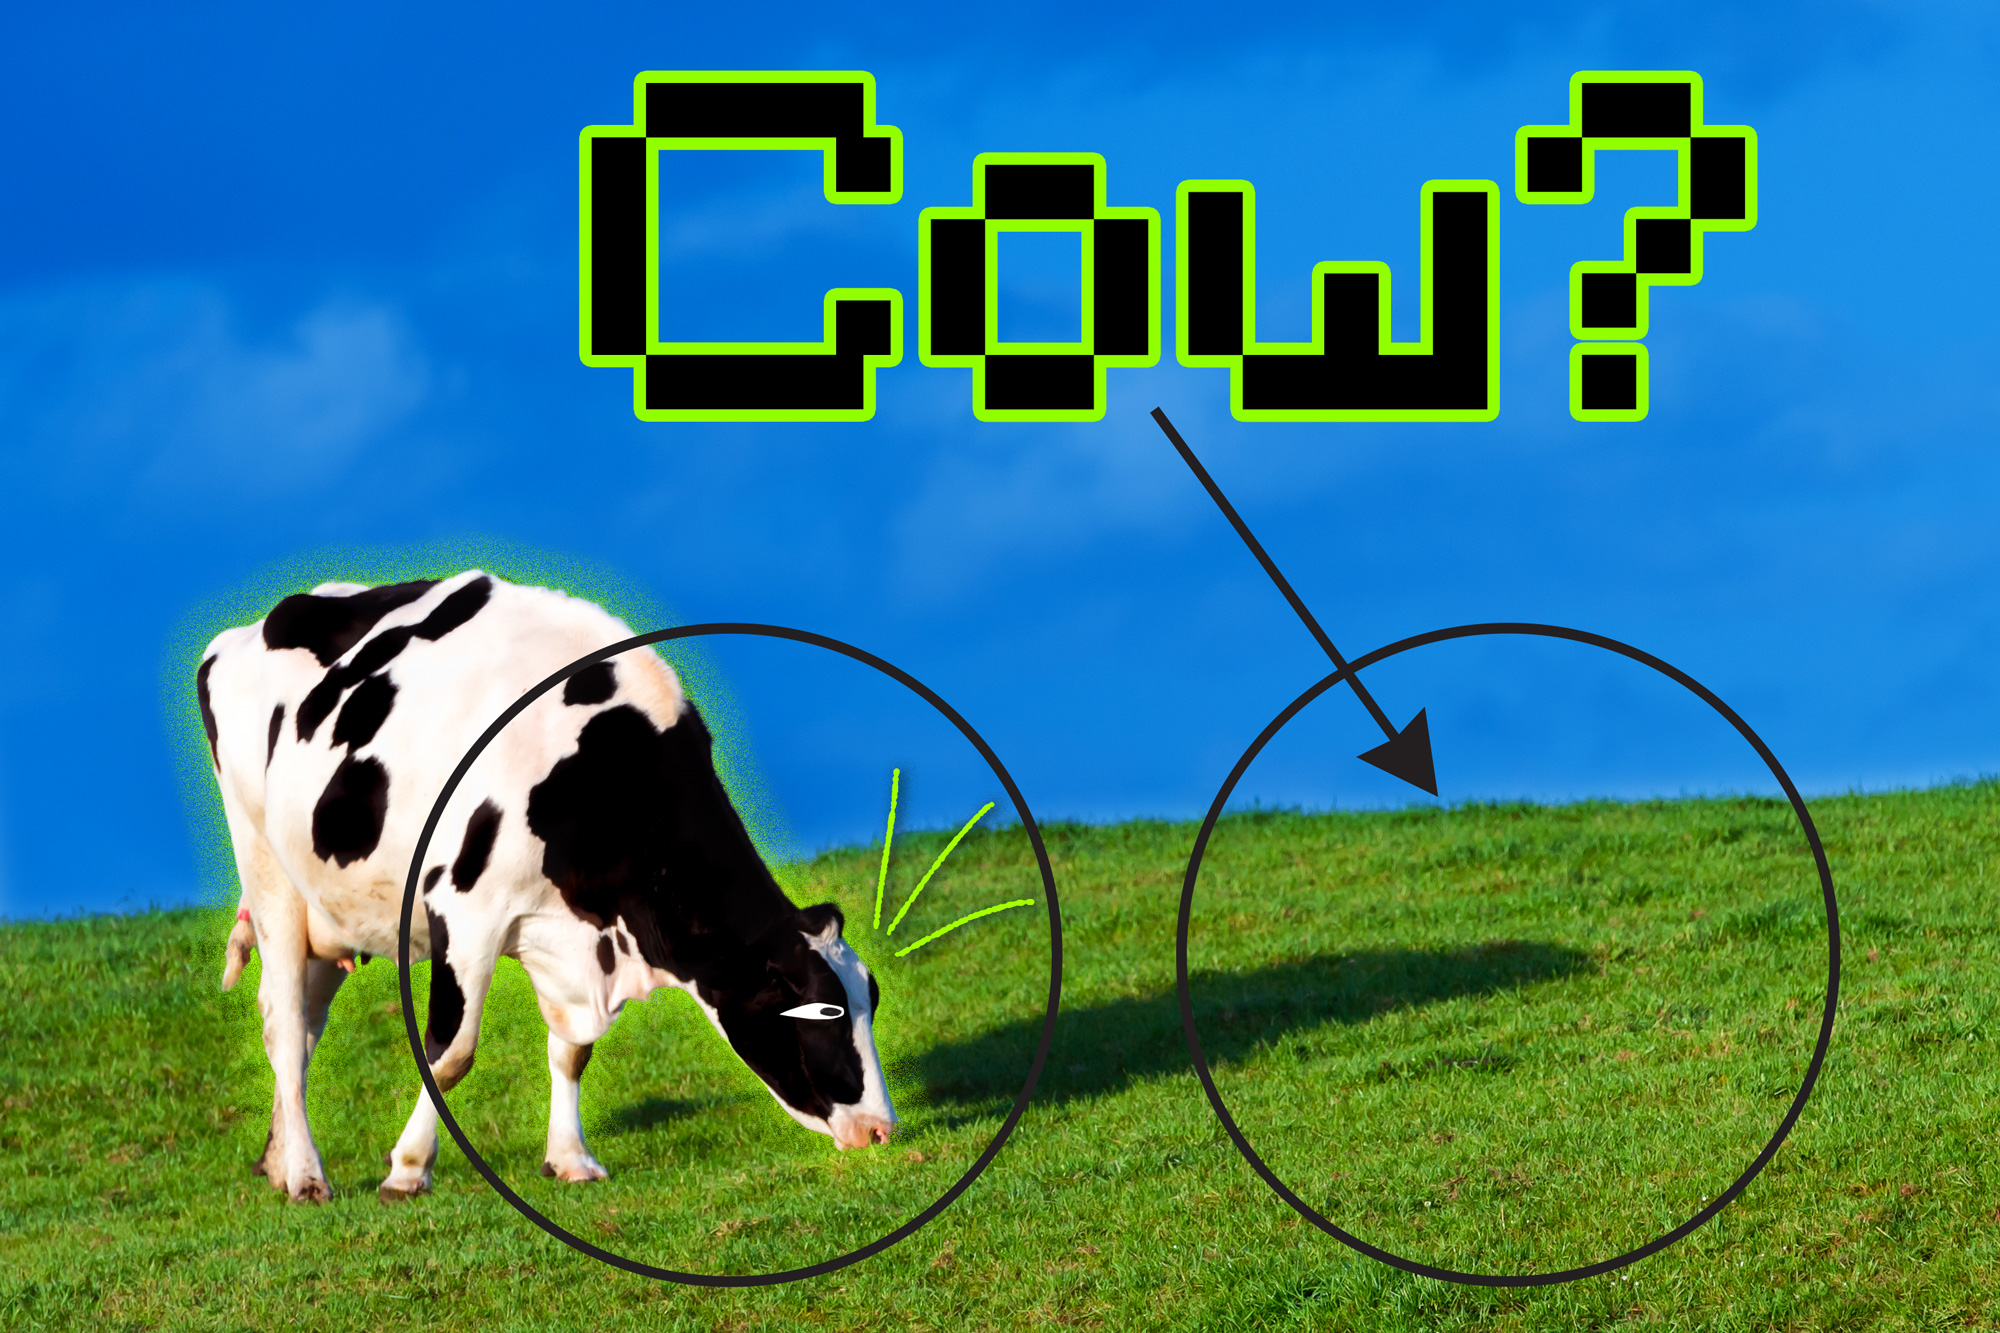
\includegraphics[width=0.95\linewidth]{photos/failure_1.jpg}
				\usebeamercolor[fg]{caption}\small 
				\textit{Fig: ERM relies on "Grass" (Shortcut) instead of the actual "Cow" geometry.}
			\end{column}
		\end{columns}
	\end{frame}

\begin{frame}{Information Bottleneck in Deep ConvNets}
		\begin{columns}[T]
			% --- CỘT TRÁI: ĐẶT VẤN ĐỀ NGẮN GỌN ---
			\begin{column}{0.40\textwidth}
    \begin{block}{The Last-Layer Problem}
        \begin{itemize}
            \item Standard CNNs use \textbf{deepest features} only.
           
        \end{itemize}
    \end{block}
    
    \begin{alertblock}{The Invariant Signal}
        \begin{itemize}
            \item \textbf{Early/Mid Layers:} Hold shapes and edges.
           
        \end{itemize}
    \end{alertblock}
 $\implies$ Corrupted by style
and filters out raw structure details.
 
\end{column}
			
			% --- CỘT PHẢI: SƠ ĐỒ KIẾN TRÚC MINH HỌA ---
			\begin{column}{0.55\textwidth}
				\centering
				\vspace{0.1cm}
				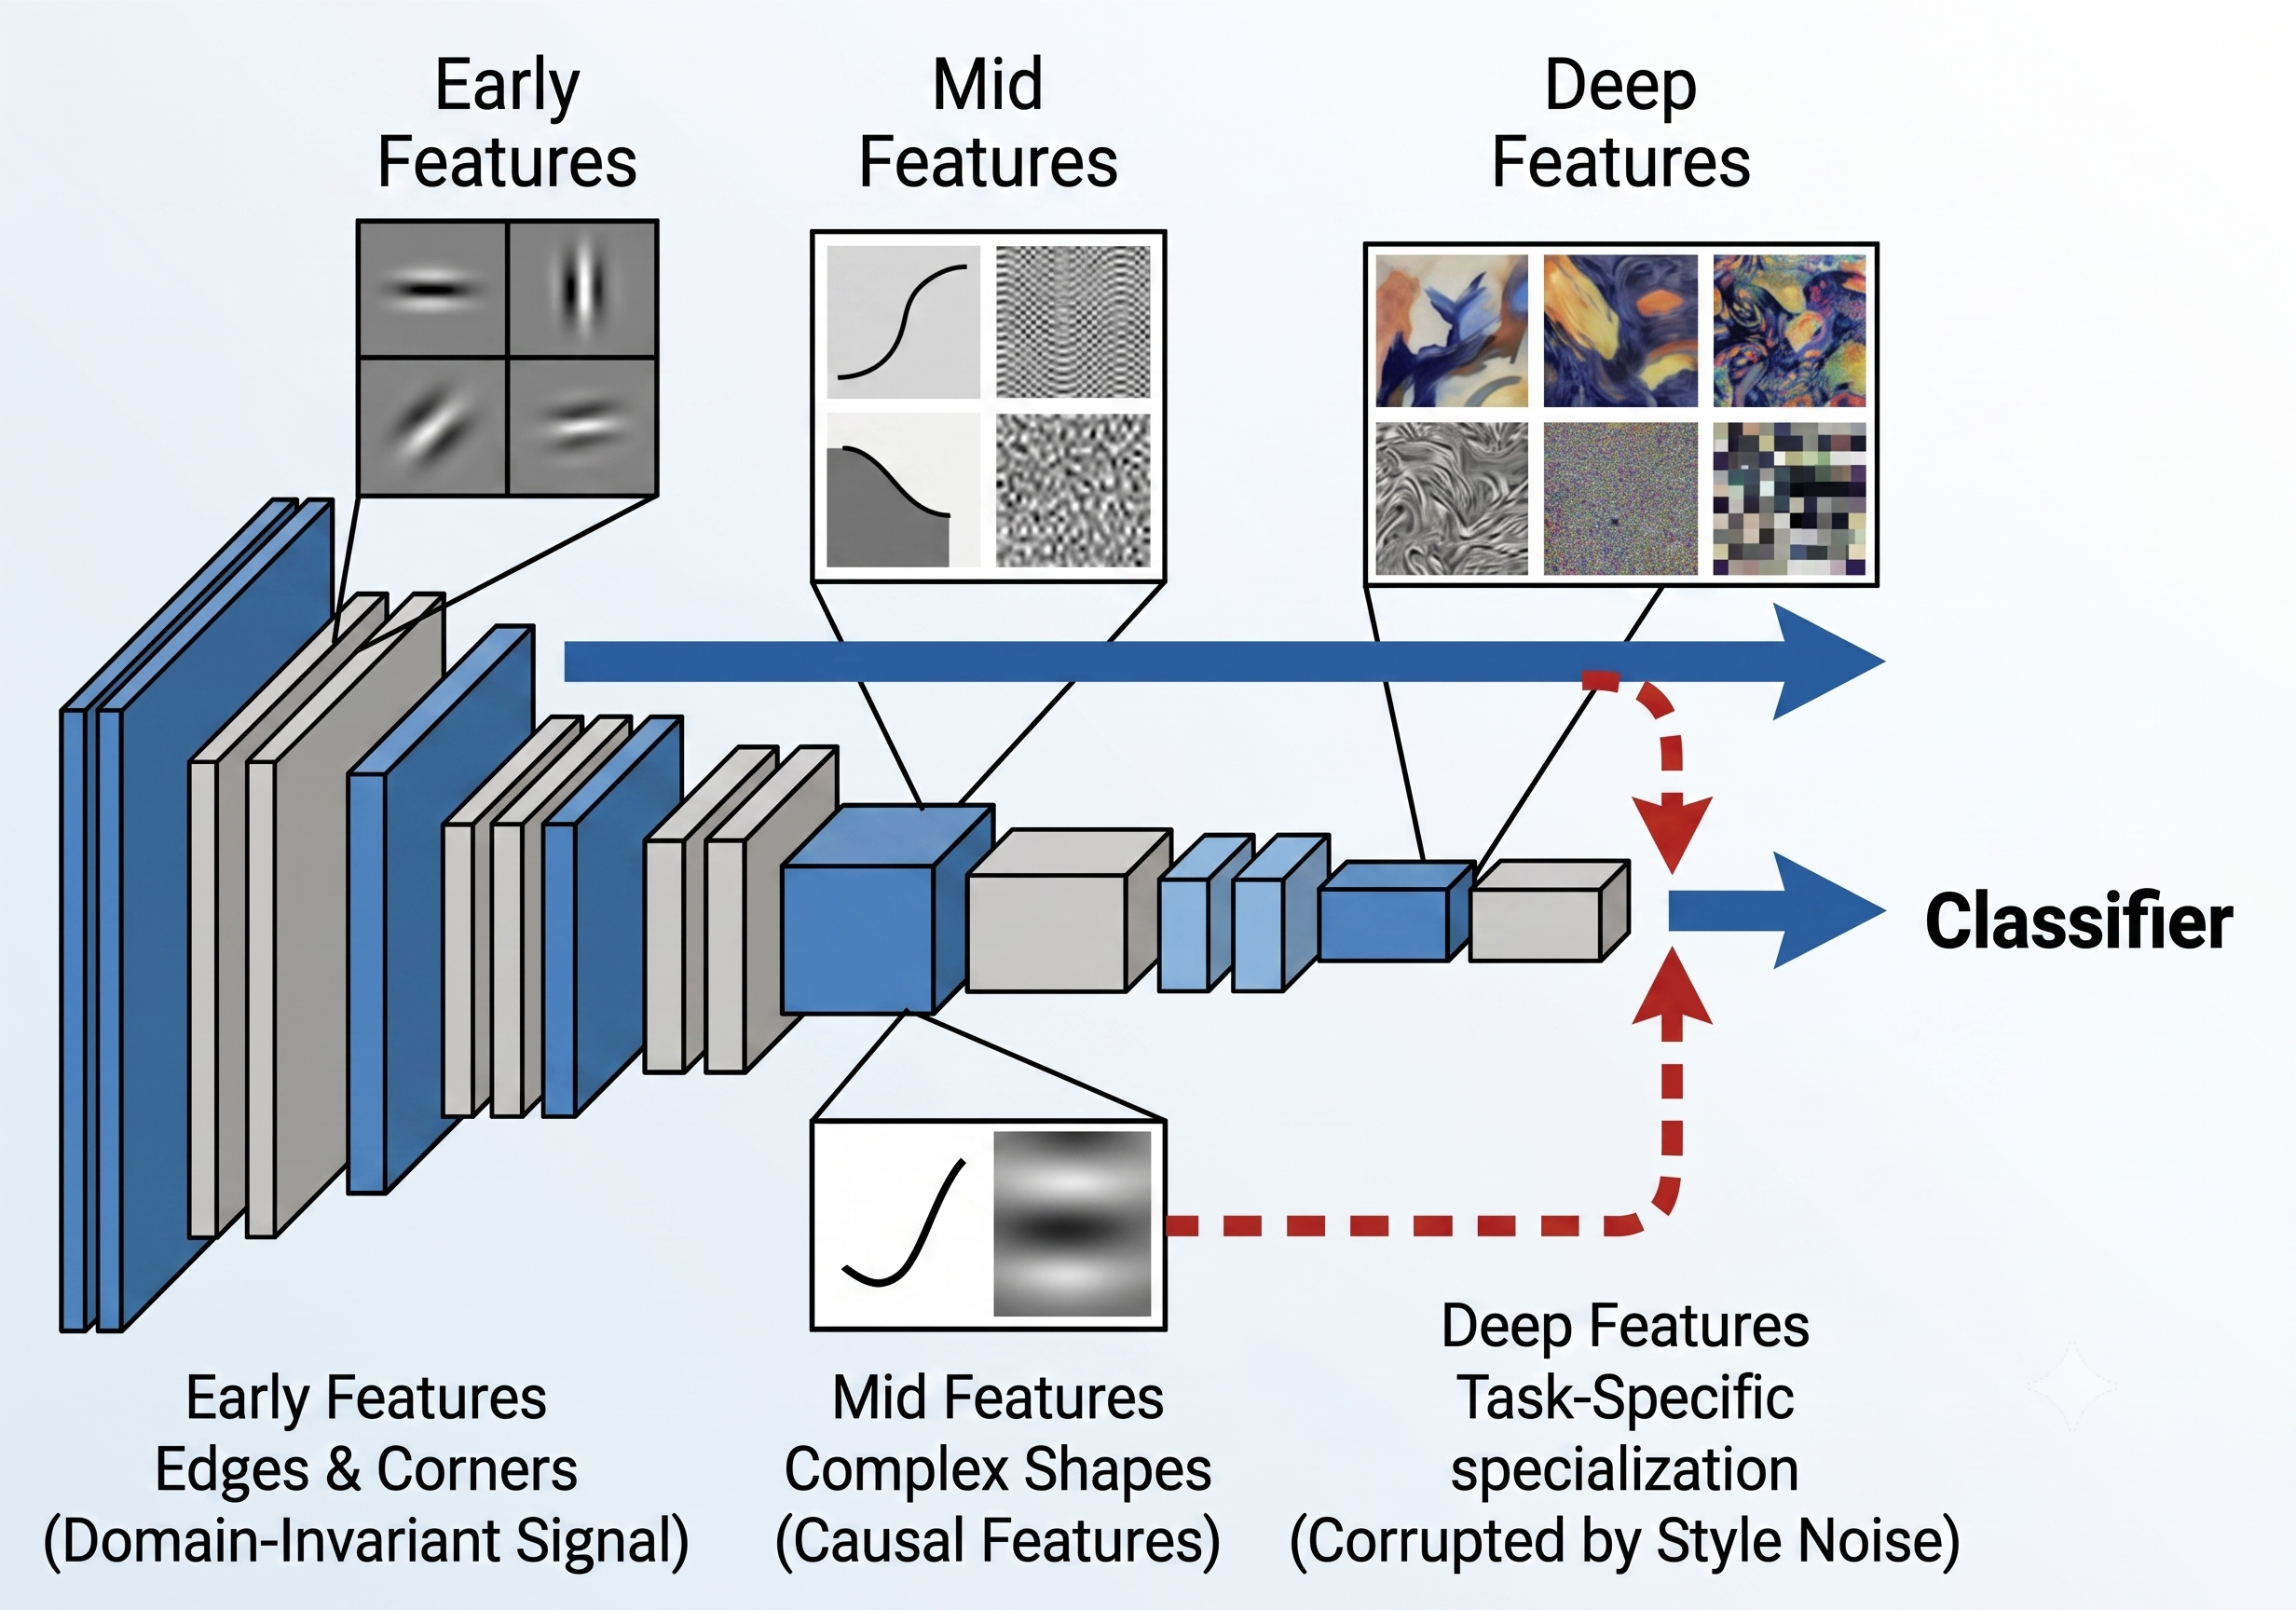
\includegraphics[width=\linewidth]{photos/bottleneck.png}
				\usebeamercolor[fg]{caption}\small 
				% \textit{Fig: Feature hierarchy in CNNs. Early layers preserve geometric shapes; Deep layers specialize in domain styles.}
			\end{column}
		\end{columns}
	\end{frame}
	% =================================================================
	% SECTION 2: THEORETICAL BACKGROUND
	% =================================================================
	% \section{Theoretical Background}

\begin{frame}{Causal vs. Style Attribute Disentanglement}
		\begin{columns}[T]
			% --- CỘT TRÁI: TỔNG QUAN VỀ SỰ TÁCH BIỆT ---
			\begin{column}{0.45\textwidth}
				\begin{block}{Latent Space Split: $X \approx (a, d)$}
					\begin{itemize}
						\item \textbf{Causal ($a$):} Class-specific \textbf{geometry}(Invariant).
						\item \textbf{Style ($d$):} Domain-specific \textbf{context} and texture (Noise).
					\end{itemize}
				\end{block}
				
				\begin{alertblock}{The DG Goal}
					Isolate \textbf{Causal $a$} from \textbf{Style $d$} to ensure the model only relies on invariant geometry for prediction.
				\end{alertblock}
			\end{column}
			
			% --- CỘT PHẢI: HÌNH ẢNH PIPELINE TÁCH BIỆT ---
			\begin{column}{0.55\textwidth}
				\centering
				\vspace{0.1cm}
				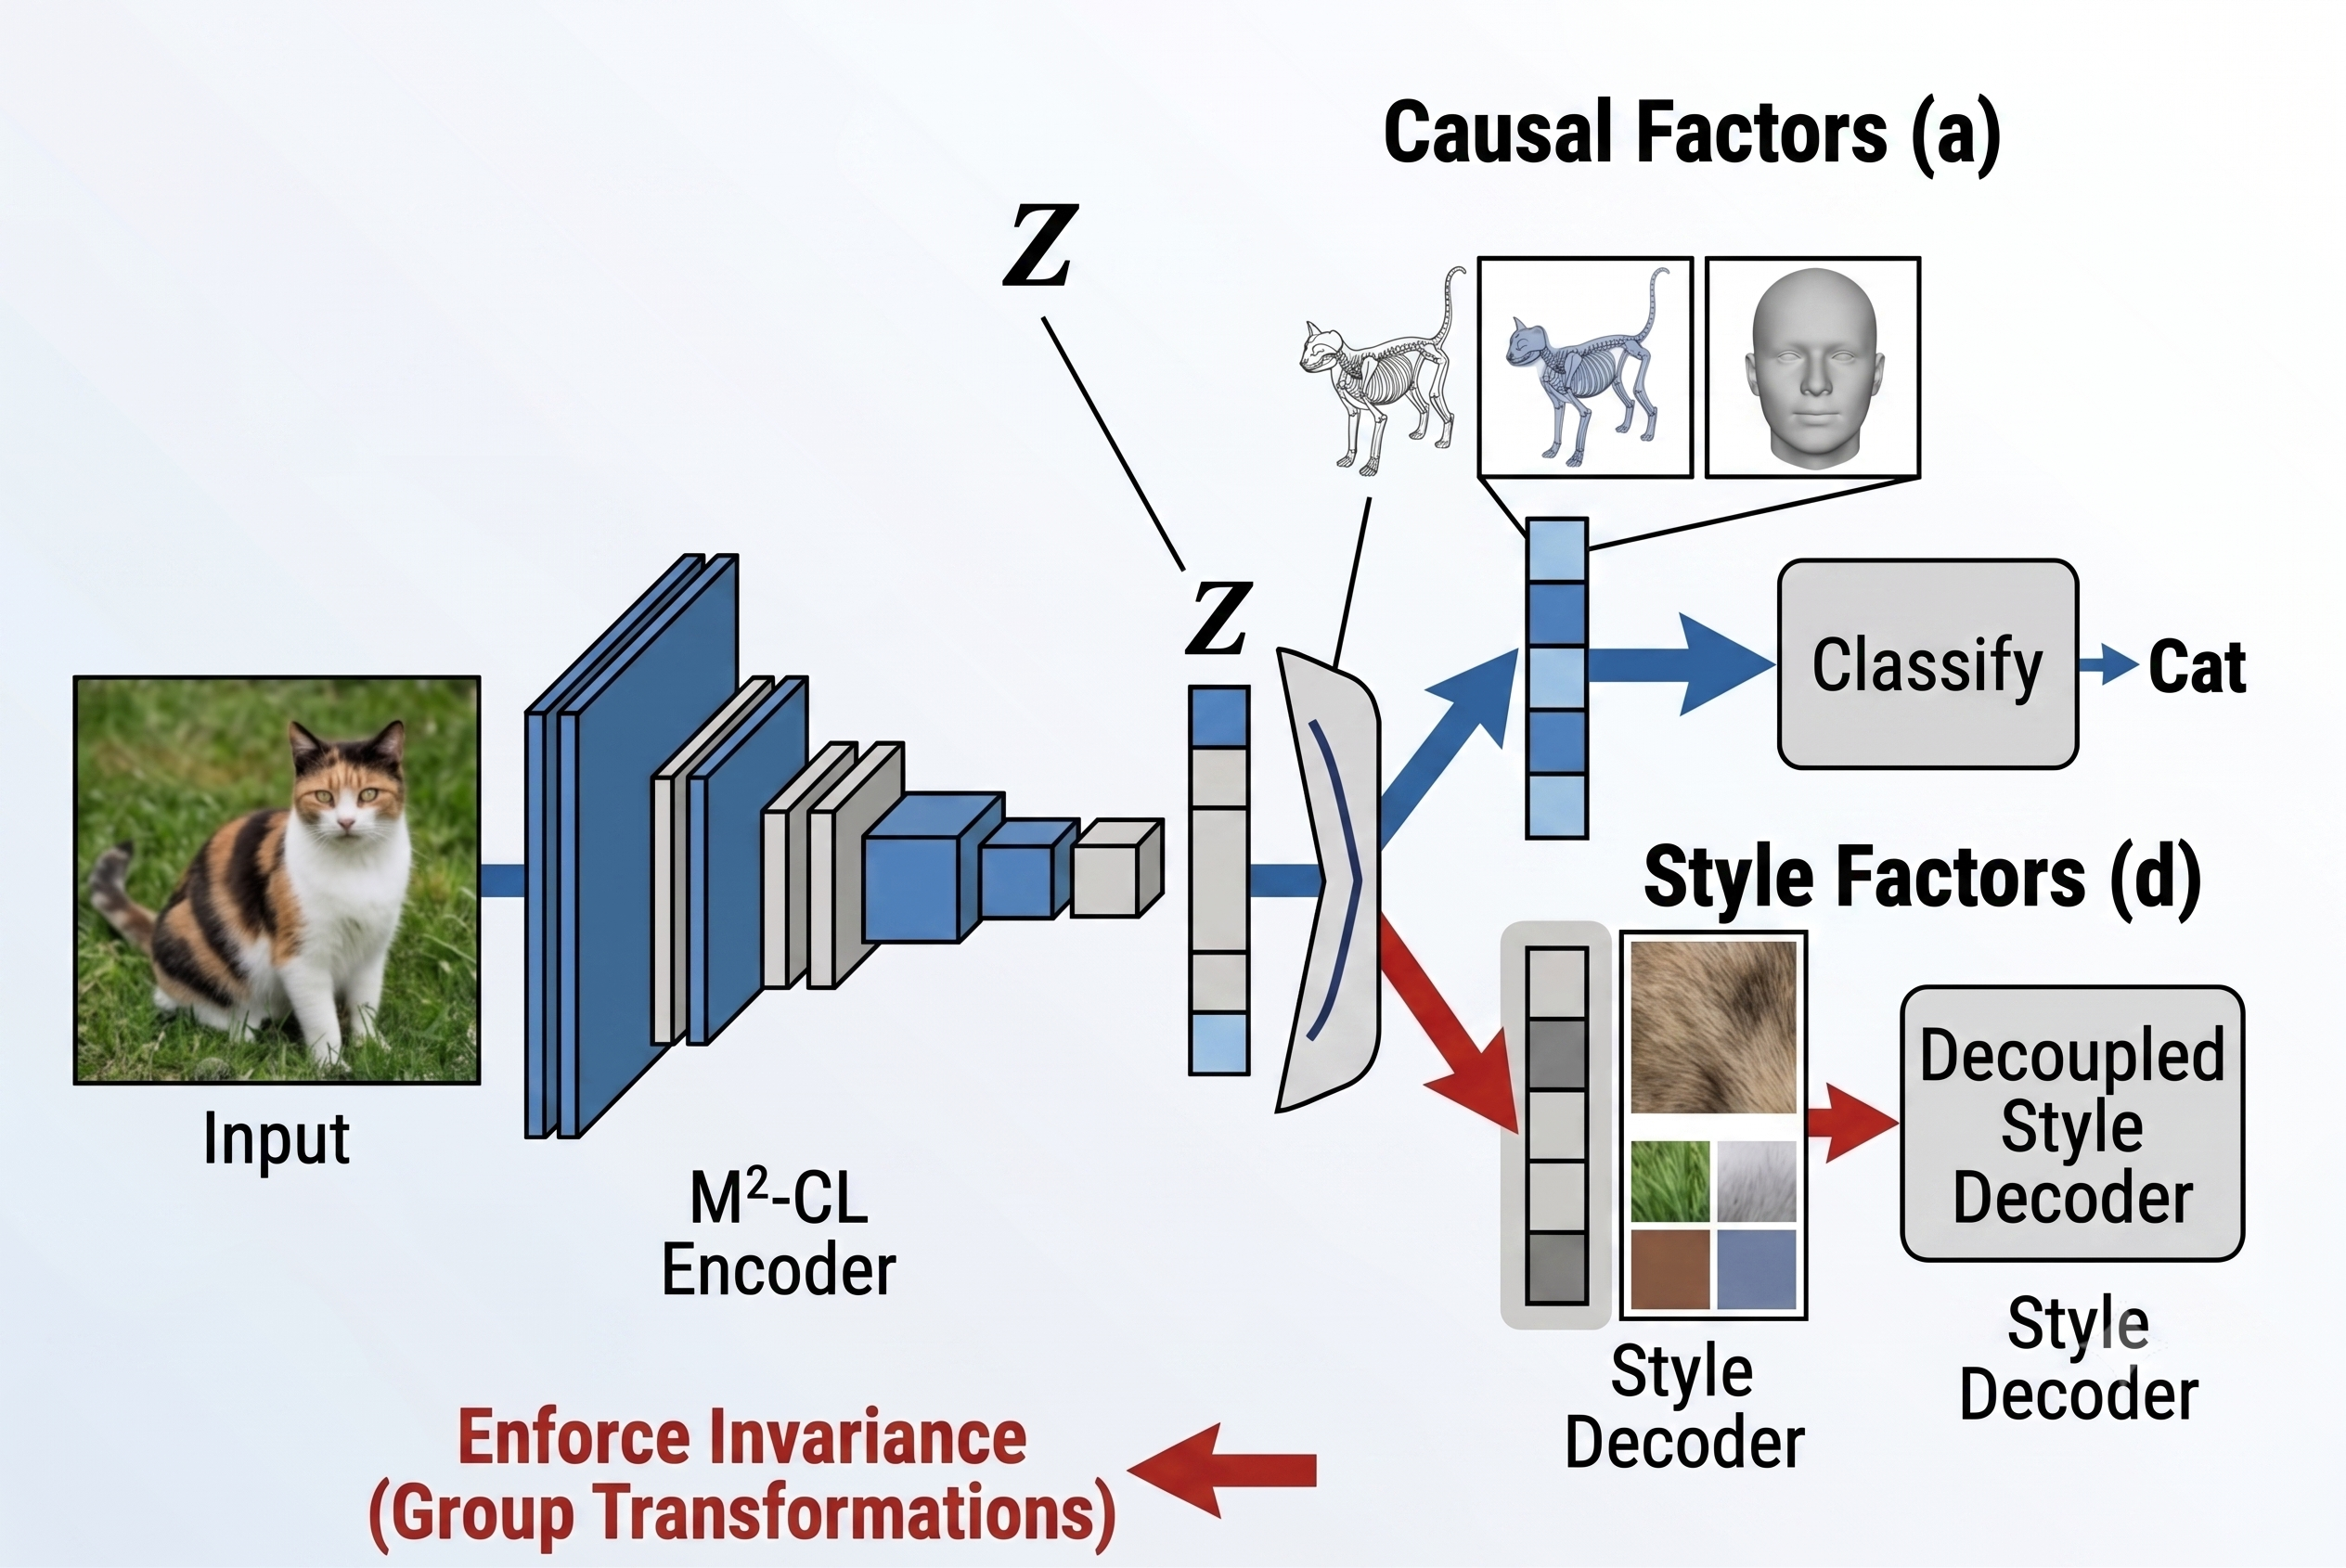
\includegraphics[width=\linewidth]{photos/disentangled.png}
				\usebeamercolor[fg]{caption}\small 
				% \textit{Fig: Pipeline disentangling Causal structure ($a$) from Domain-specific Style ($d$).}
			\end{column}
		\end{columns}
	\end{frame}
\begin{frame}{Mathematical Formalization \& Multi-Layer Hypothesis}
		\begin{columns}[T]
			% --- CỘT TRÁI: ĐỊNH NGHĨA TOÁN HỌC ---
			\begin{column}{0.5\textwidth}
				\begin{block}{Disentangled Group Actions}
					Let group $G = G_1 \times \dots \times G_n$ act on world space $X = X_1 \times \dots \times X_n$:
					$$ (g_1, \dots, g_n) \cdot (x_1, \dots, x_n) = (g_1 \cdot_1 x_1, \dots, g_n \cdot_n x_n) $$
					\small $\implies$ Each sub-space $X_i$ is strictly invariant to all subgroup actions $G_j$ ($j \neq i$).
				\end{block}
			\end{column}
			
			% --- CỘT PHẢI: GIẢ THUYẾT ĐA TẦNG ---
			\begin{column}{0.5\textwidth}
				\begin{alertblock}{The $M^2$ Latent Hypothesis}
					Instead of a single entangled final layer, we decompose intermediate hidden layers:
					$$ Z = Z_1 \times Z_2 \times \dots \times Z_{L-1} $$
					\small $\implies$ Extraction modules handle high-dimensionality and filter out redundant info.
				\end{alertblock}
			\end{column}
		\end{columns}
	\end{frame}

	% =================================================================
	% SECTION 3: M2 ARCHITECTURE DETAILS
	% =================================================================
	\section{The $M^2 - CL$ Architecture}

	\begin{frame}{The $M^2$ Architectural Paradigm}
		\begin{block}{Framework Concept}
			Leverages parallel multi-scale concentration blocks mapped across multiple intermediate layers of a standard backbone network.
		\end{block}
		\begin{figure}
			\centering
			% Đảm bảo file ảnh tồn tại trong thư mục của bạn hoặc giữ nguyên cấu trúc này
			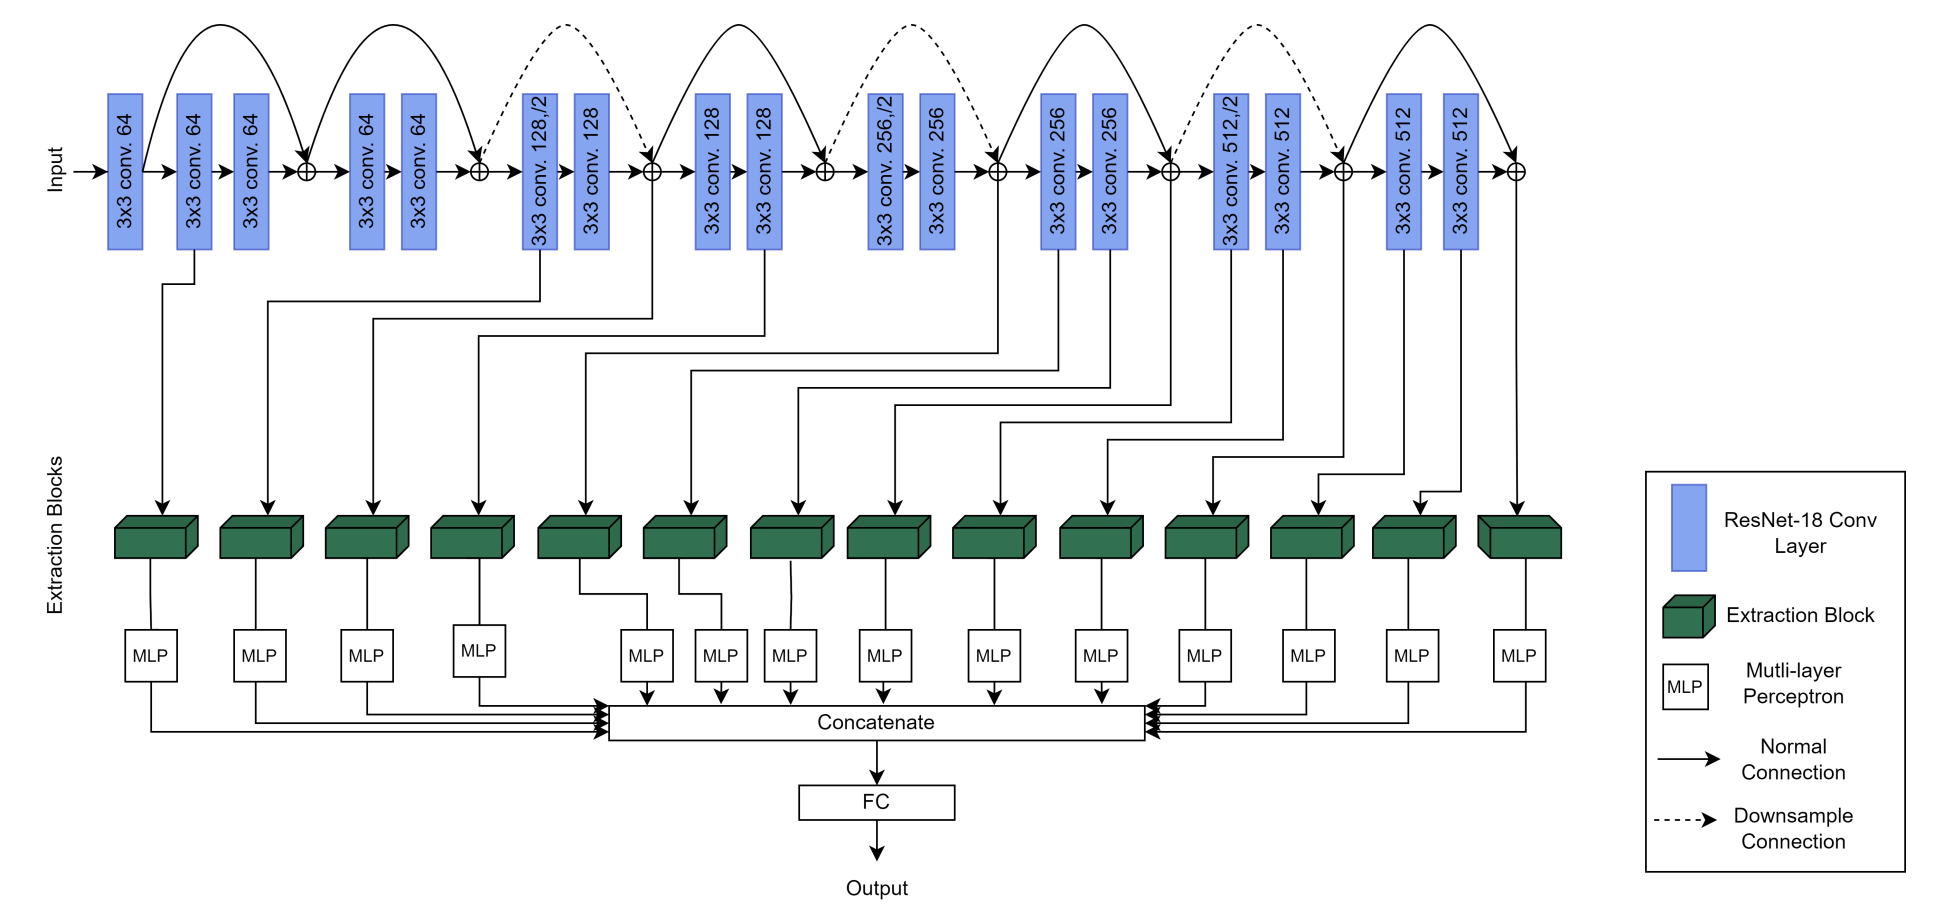
\includegraphics[width=0.75\linewidth]{photos/M2.png}
			% \caption{Visualization of the $M^2$ framework overlaid on a ResNet-18 backbone.}
			\label{fig:m2_architecture}
		\end{figure}
	\end{frame}

	\begin{frame}{Extraction Block}
		\begin{columns}[T]
			\begin{column}{0.48\textwidth}
				\begin{figure}
					\centering
					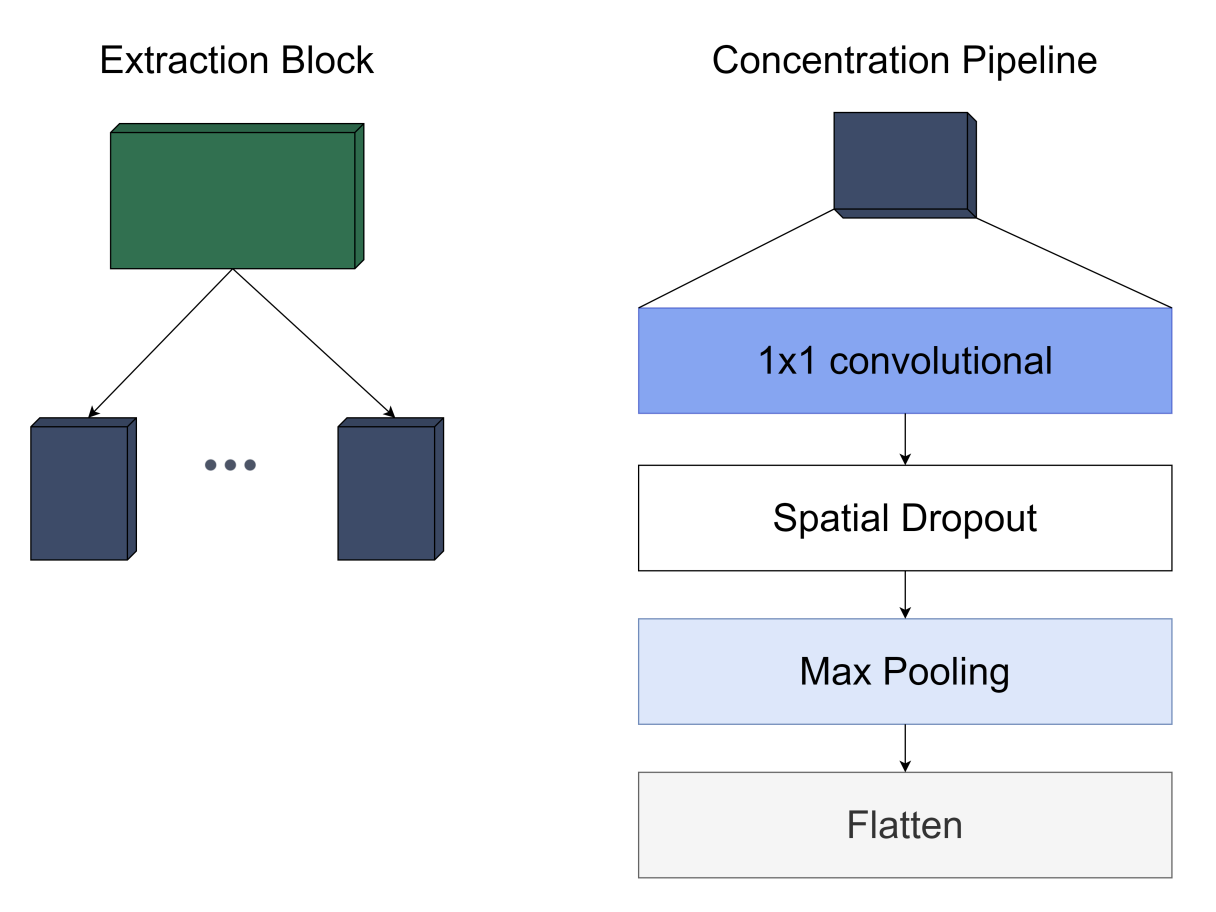
\includegraphics[width=0.9\linewidth]{photos/extraction.png}
					\caption{Concentration pipeline layout.}
				\end{figure}
			\end{column}
			\begin{column}{0.52\textwidth}
				\begin{block}{Internal Sequence Mechanics}
					\begin{enumerate}
						\item \textbf{$1\times1$ Convolutional Layer:} Compresses high-dimensional channels $c$ down to $\lfloor c/r \rfloor$ using a reduction factor $r$.
						\item \textbf{Spatial Dropout Layer:} Mitigates pixel correlation leakage.
						\item \textbf{Multi-Scale Max Pooling:} Captures spatial features before reduction.
						\item \textbf{MLP Projection Vector:} Maps pooled features into vectors via MLPs.
					\end{enumerate}
				\end{block}
			\end{column}
		\end{columns}
	\end{frame}

\begin{frame}{Spatial Dropout}
	\begin{columns}[T]
		% --- CỘT TRÁI: SO SÁNH TỪ KHÓA ---
		\begin{column}{0.45\textwidth}
			\begin{block}{Vanilla Dropout (CNN Failure)}
				\begin{itemize}
					\item Drops \textbf{individual pixels} randomly.
					\item \alert{Result:} Info leaks; regularization fails.
				\end{itemize}
			\end{block}
			
			\begin{alertblock}{Spatial Dropout (Our Solution)}
				\begin{itemize}
					\item Drops \textbf{entire feature maps} ($H \times W$).
					\item Forces network to find alternative cues.
					\item \textbf{Result:} Blocks local style shortcuts.
				\end{itemize}
			\end{alertblock}
		\end{column}
		
		% --- CỘT PHẢI: HÌNH ẢNH MINH HỌA 3D TENSOR ---
		\begin{column}{0.55\textwidth}
			\centering
			\vspace{0.3cm}
			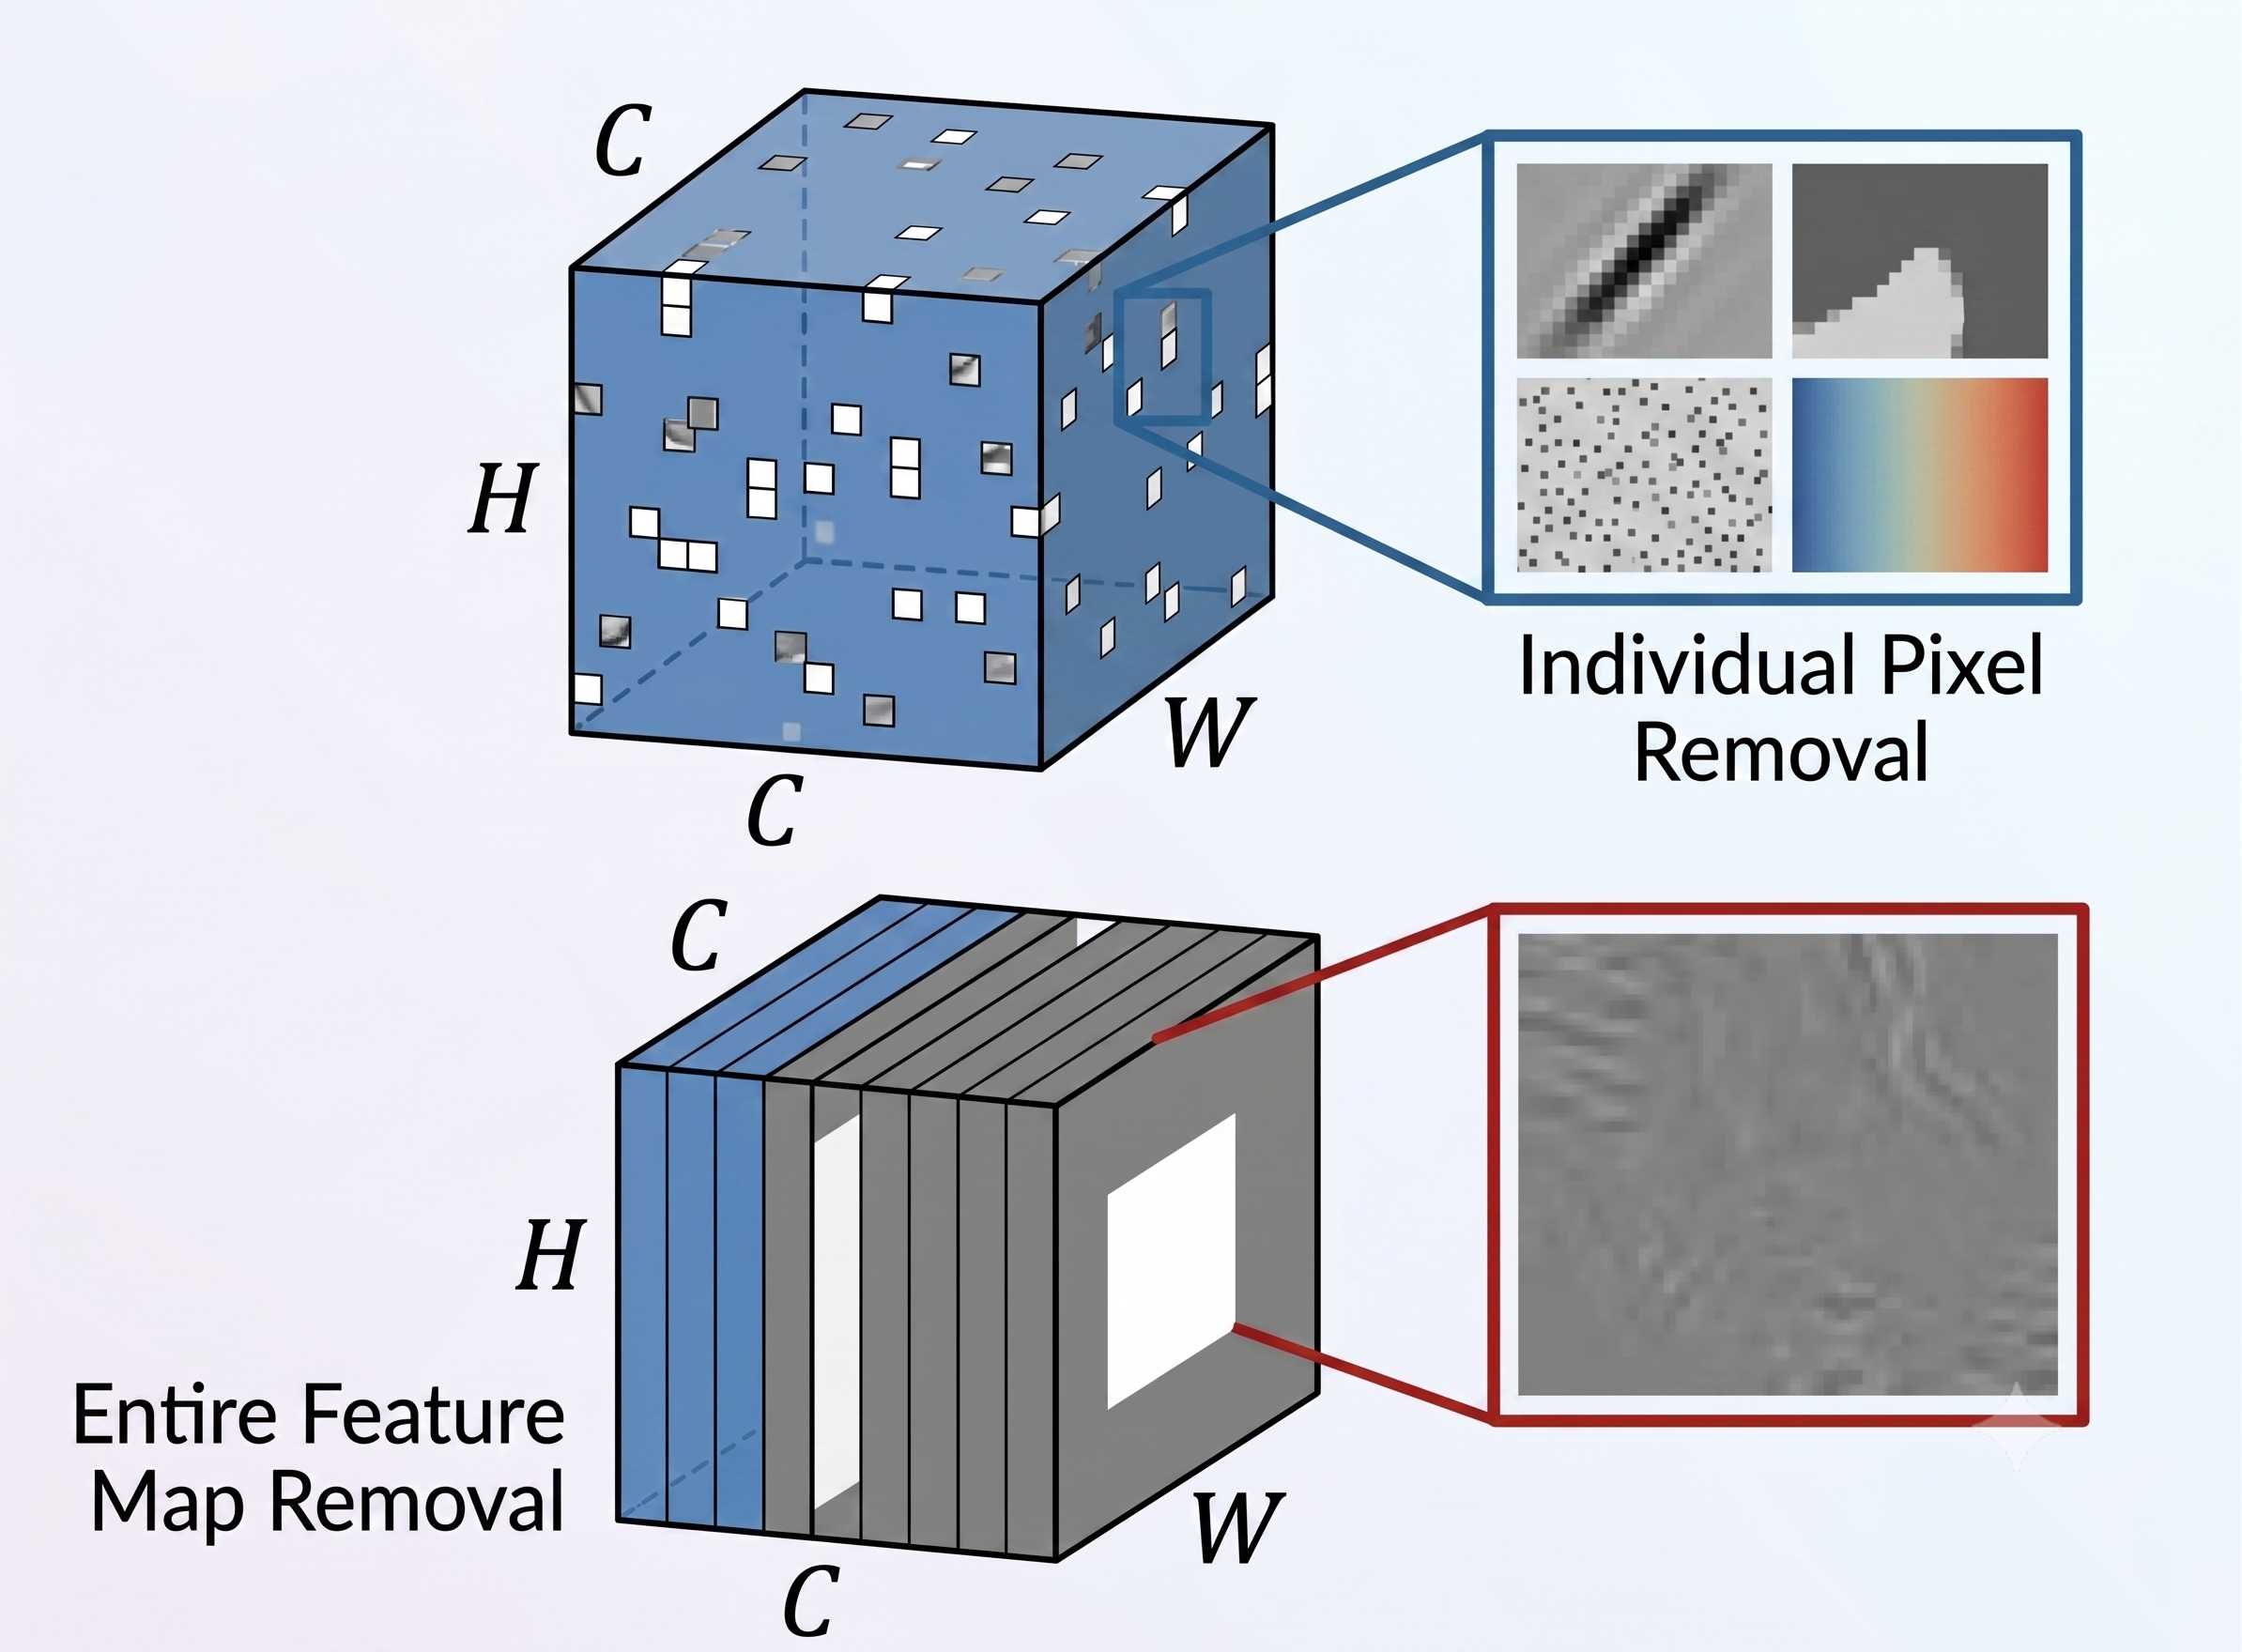
\includegraphics[width=\linewidth]{photos/spatial_dropout.png}
			\usebeamercolor[fg]{caption}\small 
			% \textit{Fig: Structural comparison. Spatial Dropout removes full 2D channels to prevent correlation leakage.}
		\end{column}
	\end{columns}
\end{frame}
\begin{frame}{Multi-Scale Concentration \& Hypercolumn Construction}
		\begin{columns}[T]
			% --- CỘT TRÁI: TEXT TINH GỌN (45% Chiều rộng) ---
			\begin{column}{0.45\textwidth}
				\begin{block}{Spatial Scaling Allocations}
					
					\begin{itemize}
						\item \textbf{Early Hooks:} Pooling sizes optimized for $8\times8$, $4\times4$, and $2\times2$.
						\item \textbf{Late Hooks:} Deeper fields adapt to $7\times7$ and $3\times3$ dimensions.
					\end{itemize}
				\end{block}
				
				\begin{alertblock}{Concatenation Protocol}
					Flattened multi-scale vectors are concatenated into a \textbf{hypercolumn vector} for final FC layer classification.
				\end{alertblock}
			\end{column}
			
			% --- CỘT PHẢI: CHÈN ẢNH MINH HỌA (55% Chiều rộng) ---
			\begin{column}{0.55\textwidth}
				\centering
				\vspace{0.2cm}
				% Thay tên file ảnh sơ đồ kiến trúc của bạn vào đây
				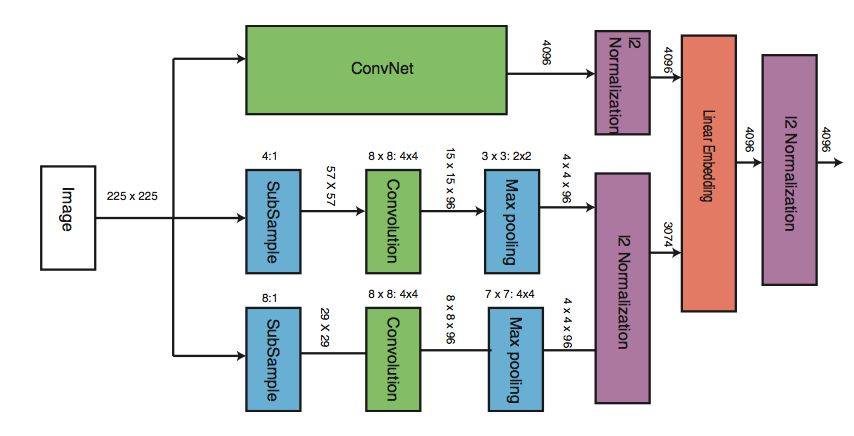
\includegraphics[width=\linewidth]{photos/multilscale.png}
				\usebeamercolor[fg]{caption}\small 
				\textit{Fig: Multi-scale pooling pipelines merging into a unified Hypercolumn vector.}
			\end{column}
		\end{columns}
	\end{frame}


	% =================================================================
	% SECTION 4: THE M2-CL LOSS FRAMEWORK
	% =================================================================
	

	\begin{frame}{Supervised Contrastive Regularization Strategy}
		\begin{block}{The Necessity of Geometric Constraints}
			Simply extracting intermediate representations does not ensure that hidden filters actively discard domain-specific style noise. 
		\end{block}
		\begin{alertblock}{Target Geometric Alignment}
			\begin{itemize}
				\item \textbf{Pull Same-Class Closely:} Force representations of identical semantic labels (e.g., a Dog in Photo and a Dog in Sketch) to align tightly in the latent space across domains.
				\item \textbf{Push Different-Classes Apart:} Move different semantic labels far apart, even if they share an identical background style.
			\end{itemize}
		\end{alertblock}
	\end{frame}

	\begin{frame}{Mathematical Formulation of Layer-Wise Loss}
		\begin{block}{Probability Alignment Measure}
			Let $u_i^{(l)}$ be the L2-normalized extraction vector ($||u_i^{(l)}||=1$) of sample $x_i$ at hidden layer $l$. The probability alignment measure of class $c$ within a batch is defined as:
			$$ p^{(l)}(c) = \frac{\sum_{i=1}^{N_c}\sum_{j=i+1}^{N_c} \exp(u_i^{(l)T}u_j^{(l)} / \tau)}{\sum_{i=1}^{N_b}\sum_{a \neq i}^{N_b}\exp(u_i^{(l)T}u_a^{(l)} / \tau)} $$
		\end{block}
		\begin{alertblock}{Parameters Key}
			\begin{itemize}
				\item $N_c$: Total count of elements belonging strictly to class $c$ inside the batch.
				\item $N_b$: Complete batch sample size count.
				\item $\tau$: Temperature parameter regulating distribution density mass.
			\end{itemize}
		\end{alertblock}
	\end{frame}

	\begin{frame}{The Total Optimization Objective}
		\begin{block}{Joint Structural Loss}
			Considering all $C$ distinct classes, the total log-likelihood regularizer loss over $M$ selected hidden layers is formulated as:
			$$ \mathcal{L}^{(l)} = -\sum_{c=1}^{C}\log p^{(l)}(c) \implies \mathcal{L} = \mathcal{L}_{CE} + \alpha \sum_{l=1}^{M}\mathcal{L}^{(l)} $$
		\end{block}
		\begin{alertblock}{Hyperparameter Definition}
			\begin{itemize}
				\item $\mathcal{L}_{CE}$: Classical cross-entropy loss driving target category discrimination.
				\item $\alpha$: Scaling weight setting the optimization magnitude of the contrastive regularization branch.
			\end{itemize}
		\end{alertblock}
	\end{frame}

\begin{frame}{Computational Efficiency Principles}
	\begin{block}{The Bottleneck}
		Pairwise vector products across multiple hidden layers $\implies$ \alert{Severe memory bottlenecks}.
	\end{block}
	\begin{alertblock}{The Matrix Parallelization Solution}
		\begin{itemize}
			\item \textbf{Instant Computation:} Stack batch vectors into matrix $U^{(l)} \rightarrow U^{(l)T}U^{(l)}$.
			\item \textbf{Minimal Overhead:} Denominator computed \textbf{once per batch} (identical for all classes).
		\end{itemize}
	\end{alertblock}
\end{frame}

	% =================================================================
	% SECTION 5: EXPERIMENTAL SETUP
	% =================================================================
	\section{Experimental}
	\useStyleLogoOnly
	\useThickBar

	\begin{frame}{Technical Specifications \& Hyperparameters}
		\begin{alertblock}{Optimizer Configurations}
			\begin{itemize}
				\item Base Optimization: Stochastic Gradient Descent (SGD) for 30 epochs.
				\item Learning Rate: 0.001, Batch Size Allocation: 128.
				\item Default Extraction Blocks Settings: Reduction factor $r=4$.
				\item Default Loss Balancing: Weight $\alpha = 0.01$, Temperature $\tau = 1.0$.
			\end{itemize}
		\end{alertblock}
	\end{frame}

	\begin{frame}{Evaluation Benchmarks}
		\begin{columns}[T]
			% --- CỘT 1: PACS ---
            	\begin{column}{0.33\textwidth}
				\begin{alertblock}{VLCS Dataset}
					\begin{itemize}
						\item \textbf{Size:} 10,729 images | \textbf{Classes:} 5
						\item \textbf{Domains (4):} PASCAL, LabelMe, Caltech, SUN.
					\end{itemize}
				\end{alertblock}
				\centering
				\vspace{0.1cm}
				
			\end{column}
			\begin{column}{0.33\textwidth}
				\begin{block}{PACS Dataset}
					\begin{itemize}
						\item \textbf{Size:} 9,991 images | \textbf{Classes:} 7
						\item \textbf{Domains (4):} Photo, Art Painting, Cartoon, Sketch.
					\end{itemize}
				\end{block}
				\centering
				\vspace{0.1cm}
				
			\end{column}
			
			% --- CỘT 2: VLCS ---
		
			
			% --- CỘT 3: OFFICE-HOME ---
			\begin{column}{0.33\textwidth}
				\begin{block}{Office-Home Dataset}
					\begin{itemize}
						\item \textbf{Size:} 15,588 images | \textbf{Classes:} 65
						\item \textbf{Domains (4):} Art, Clipart, Product, Real-World.
					\end{itemize}
				\end{block}
				\centering
				\vspace{0.1cm}
				
			\end{column}
		\end{columns}
    \begin{figure}
        \centering
        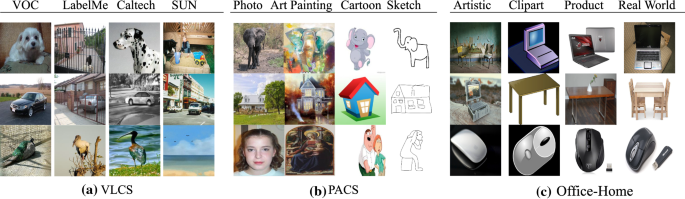
\includegraphics[width=0.65\linewidth]{photos/dataset_cv1.png}
        \label{fig:placeholder}
    \end{figure}
	\end{frame}

	

	% =================================================================
	% SECTION 6: QUANTITATIVE RESULTS & ABLATIONS
	% =================================================================
	% \section{Quantitative Results \& Analysis}

	\begin{frame}{Training Convergence on PACS (ResNet-18)}
		\begin{figure}
			\centering
			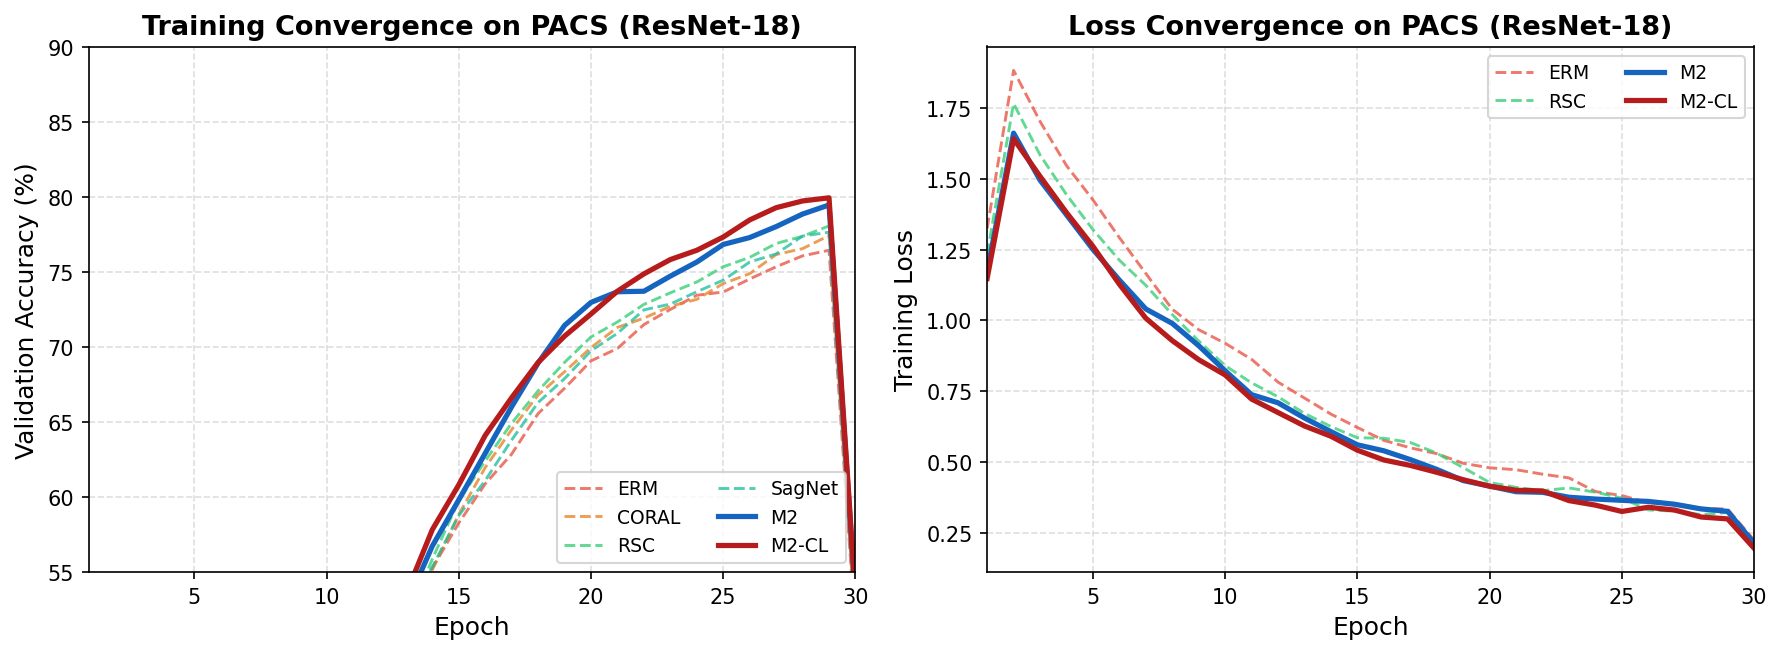
\includegraphics[width=0.92\linewidth]{photos/training_curves.png}
		\end{figure}
		\vspace{-0.3cm}
		\begin{block}{}
			\small $M^2$-CL converges faster and plateaus \textbf{higher} than all baselines. The contrastive regularizer suppresses loss spikes caused by domain-conflicting gradients.
		\end{block}
	\end{frame}

	\begin{frame}{Dataset Table 1: PACS and VLCS (ResNet-18)}
\begin{table}[htbp]
\centering
\caption{Top-1 accuracy on PACS and VLCS, ResNet-18.}
\scriptsize
\begin{adjustbox}{max width=\textwidth}
\begin{tabular}{lrrrrrrrrrr}
\toprule
Method & Art & Cartoon & Photo & Sketch & Avg & Caltech & Labelme & Sun & Voc & Avg \\
\midrule
ERM & 76.53 & 74.80 & 94.95 & 67.89 & 78.54 & 96.87 & 65.03 & 71.62 & 71.60 & 76.28 \\
RSC & 79.26 & 76.12 & 95.07 & 70.88 & 80.34 & 97.68 & 66.33 & 73.53 & 72.75 & 77.57 \\
CORAL & 78.55 & 72.74 & 92.24 & 73.93 & 79.36 & 95.16 & 60.73 & 70.66 & 65.00 & 72.89 \\
MIXUP & 79.79 & 72.81 & 93.11 & 63.97 & 77.42 & 93.44 & 60.25 & \textbf{74.36} & 69.87 & 74.48 \\
MMD & 77.75 & 73.35 & 92.34 & 69.74 & 78.29 & 97.28 & 60.62 & 70.48 & 65.21 & 73.40 \\
SagNet & 78.71 & 74.90 & 94.79 & 70.48 & 79.72 & 95.76 & 61.22 & 69.61 & 71.90 & 74.62 \\
SelfReg & 79.46 & 76.32 & \textbf{95.93} & 71.60 & 80.83 & 92.53 & 62.56 & 70.27 & 72.15 & 74.38 \\
ARM & 79.77 & 75.33 & 94.43 & \underline{74.76} & 81.07 & 95.86 & 60.19 & 70.66 & 72.83 & 74.89 \\
EQRM & 78.61 & 72.38 & 92.48 & 71.13 & 78.65 & 96.17 & 60.57 & 70.44 & 64.66 & 72.96 \\
SAGM & 78.22 & 75.14 & 94.79 & 70.46 & 79.65 & 96.37 & 66.22 & 71.14 & 71.35 & 76.27 \\
\midrule
\textbf{M2} & \underline{80.64} & \underline{76.91} & 95.50 & 74.20 & \underline{81.81} & \underline{98.24} & \underline{67.02} & 73.80 & \underline{72.92} & \underline{78.00} \\
\textbf{M2-CL} & \textbf{81.04} & \textbf{77.48} & \underline{95.70} & \textbf{75.81} & \textbf{82.51} & \textbf{98.69} & \textbf{67.48} & \underline{74.05} & \textbf{73.76} & \textbf{78.50} \\
\bottomrule
\end{tabular}
\end{adjustbox}
\end{table}
	\end{frame}

	\begin{frame}{Dataset Table 2: PACS and VLCS (ResNet-50)}
\begin{table}[htbp]
\centering
\caption{Top-1 accuracy on PACS and VLCS, ResNet-50.}
\scriptsize
\begin{adjustbox}{max width=\textwidth}
\begin{tabular}{lrrrrrrrrrr}
\toprule
Method & Art & Cartoon & Photo & Sketch & Avg & Caltech & Labelme & Sun & Voc & Avg \\
\midrule
ERM & 83.54 & 78.47 & 96.51 & 73.64 & 83.04 & 97.01 & 62.22 & 71.79 & 76.09 & 76.78 \\
RSC & 82.08 & \textbf{80.26} & 96.51 & 75.45 & 83.57 & \textbf{97.81} & 64.44 & 74.60 & 75.53 & 78.10 \\
CORAL & 83.94 & 79.27 & 94.37 & \textbf{81.98} & 84.89 & 97.01 & 61.34 & 75.26 & 71.74 & 76.34 \\
MIXUP & 85.16 & 77.40 & 96.23 & 78.26 & 84.26 & 96.94 & 62.33 & 73.40 & 72.32 & 76.25 \\
MMD & 82.21 & 74.70 & 92.89 & 69.00 & 79.70 & 97.48 & 63.85 & 75.49 & 71.65 & 77.12 \\
SagNet & 85.23 & 78.47 & 93.20 & 77.71 & 83.65 & 94.14 & 60.43 & 70.49 & 69.96 & 73.75 \\
SelfReg & 83.33 & 79.06 & 93.16 & 77.24 & 83.20 & 92.49 & 60.73 & 66.80 & 73.58 & 73.40 \\
ARM & 82.14 & 79.10 & 92.97 & 73.02 & 81.81 & 96.01 & 63.98 & 66.26 & 71.79 & 74.51 \\
EQRM & 84.98 & 77.74 & 91.26 & 74.88 & 82.21 & 94.35 & 60.80 & 66.35 & 72.94 & 73.61 \\
SAGM & 81.35 & 78.99 & 93.24 & 79.39 & 83.24 & 97.39 & 64.23 & 69.30 & 76.17 & 76.77 \\
\midrule
\textbf{M2} & \underline{86.02} & 79.90 & \underline{97.03} & 81.50 & \underline{86.11} & 97.52 & \underline{64.77} & \underline{76.02} & \underline{76.72} & \underline{78.76} \\
\textbf{M2-CL} & \textbf{86.48} & \underline{80.05} & \textbf{97.99} & \underline{81.70} & \textbf{86.56} & \underline{97.60} & \textbf{64.86} & \textbf{76.65} & \textbf{77.26} & \textbf{79.09} \\
\bottomrule
\end{tabular}
\end{adjustbox}
\end{table}
	\end{frame}

	\begin{frame}{Performance Metrics on PACS and VLCS}
		% \begin{alertblock}{Key Analysis Takeaways}
			\begin{itemize}
				\item \textbf{State-of-the-Art:} $M^2$-CL sets a new state-of-the-art benchmark average across both backbones.
				\item \textbf{The Contrastive Loss Boost:} $M^2$-CL consistently outperforms the plain $M^2$ architecture, confirming that its explicit geometric alignment helps.
				\item \textbf{The Sketch Challenge Exception:} Performance drops slightly in the Sketch target domain[cite: 362]. This is likely because the dominant white backgrounds make it difficult for the network to separate structural objects from the domain style[cite: 363].
			\end{itemize}
		% \end{alertblock}
	\end{frame}

	\begin{frame}{Dataset Table 3: Office-Home (ResNet-18)}
\begin{table}[htbp]
\centering
\caption{Top-1 accuracy on Office-Home, ResNet-18.}
\scriptsize
\begin{adjustbox}{max width=\textwidth}
\begin{tabular}{lrrrrr}
\toprule
Method & Art & Clipart & Product & Real-World & Avg \\
\midrule
ERM & 56.12 & 47.88 & \underline{72.47} & 73.58 & 62.51 \\
RSC & 56.00 & 46.09 & 70.85 & 72.32 & 61.31 \\
CORAL & 55.46 & 49.39 & 71.75 & 73.28 & 62.47 \\
MIXUP & 56.37 & \underline{49.81} & 70.87 & 73.61 & 62.66 \\
MMD & 55.67 & 48.52 & 71.68 & 73.19 & 62.27 \\
SagNet & 55.75 & 47.74 & 71.71 & 73.17 & 62.09 \\
SelfReg & 57.56 & 49.69 & 72.43 & 73.72 & 63.35 \\
ARM & 54.47 & 48.45 & 71.14 & \underline{73.79} & 61.96 \\
EQRM & 56.08 & 48.34 & 71.57 & 72.94 & 62.23 \\
SAGM & 55.79 & 46.51 & 71.16 & 73.15 & 61.65 \\
\midrule
\textbf{M2} & \underline{58.04} & 49.30 & \textbf{73.04} & 73.50 & \underline{63.47} \\
\textbf{M2-CL} & \textbf{58.77} & \textbf{50.86} & 72.20 & \textbf{74.91} & \textbf{64.18} \\
\bottomrule
\end{tabular}
\end{adjustbox}
\end{table}
	\end{frame}

	\begin{frame}{Dataset Table 4: Office-Home (ResNet-50)}
\begin{table}[htbp]
\centering
\caption{Top-1 accuracy on Office-Home, ResNet-50.}
\scriptsize
\begin{adjustbox}{max width=\textwidth}
\begin{tabular}{lrrrrr}
\toprule
Method & Art & Clipart & Product & Real-World & Avg \\
\midrule
ERM & 63.43 & 51.32 & 76.45 & \underline{78.13} & 67.33 \\
RSC & 62.64 & 51.55 & 75.11 & 77.34 & 66.66 \\
CORAL & 61.27 & \underline{54.34} & 73.35 & 77.83 & 66.70 \\
MIXUP & 63.23 & 51.91 & \underline{77.10} & 76.39 & 67.16 \\
MMD & 59.63 & 49.37 & 75.28 & 74.71 & 64.75 \\
SagNet & 61.41 & 51.85 & 72.85 & 73.79 & 64.97 \\
SelfReg & 59.95 & 51.22 & 71.28 & 74.52 & 64.24 \\
ARM & 54.23 & 52.14 & 71.73 & 71.26 & 62.34 \\
EQRM & 63.52 & 52.32 & 73.28 & 76.45 & 66.39 \\
SAGM & 61.01 & 53.27 & 74.81 & 77.00 & 66.52 \\
\midrule
\textbf{M2} & \underline{65.35} & 53.90 & 76.80 & \textbf{78.74} & \underline{68.70} \\
\textbf{M2-CL} & \textbf{66.46} & \textbf{54.82} & \textbf{78.24} & 77.85 & \textbf{69.34} \\
\bottomrule
\end{tabular}
\end{adjustbox}
\end{table}
	\end{frame}

	\begin{frame}{Method Comparison — All Datasets (ResNet-18)}
		\begin{figure}
			\centering
			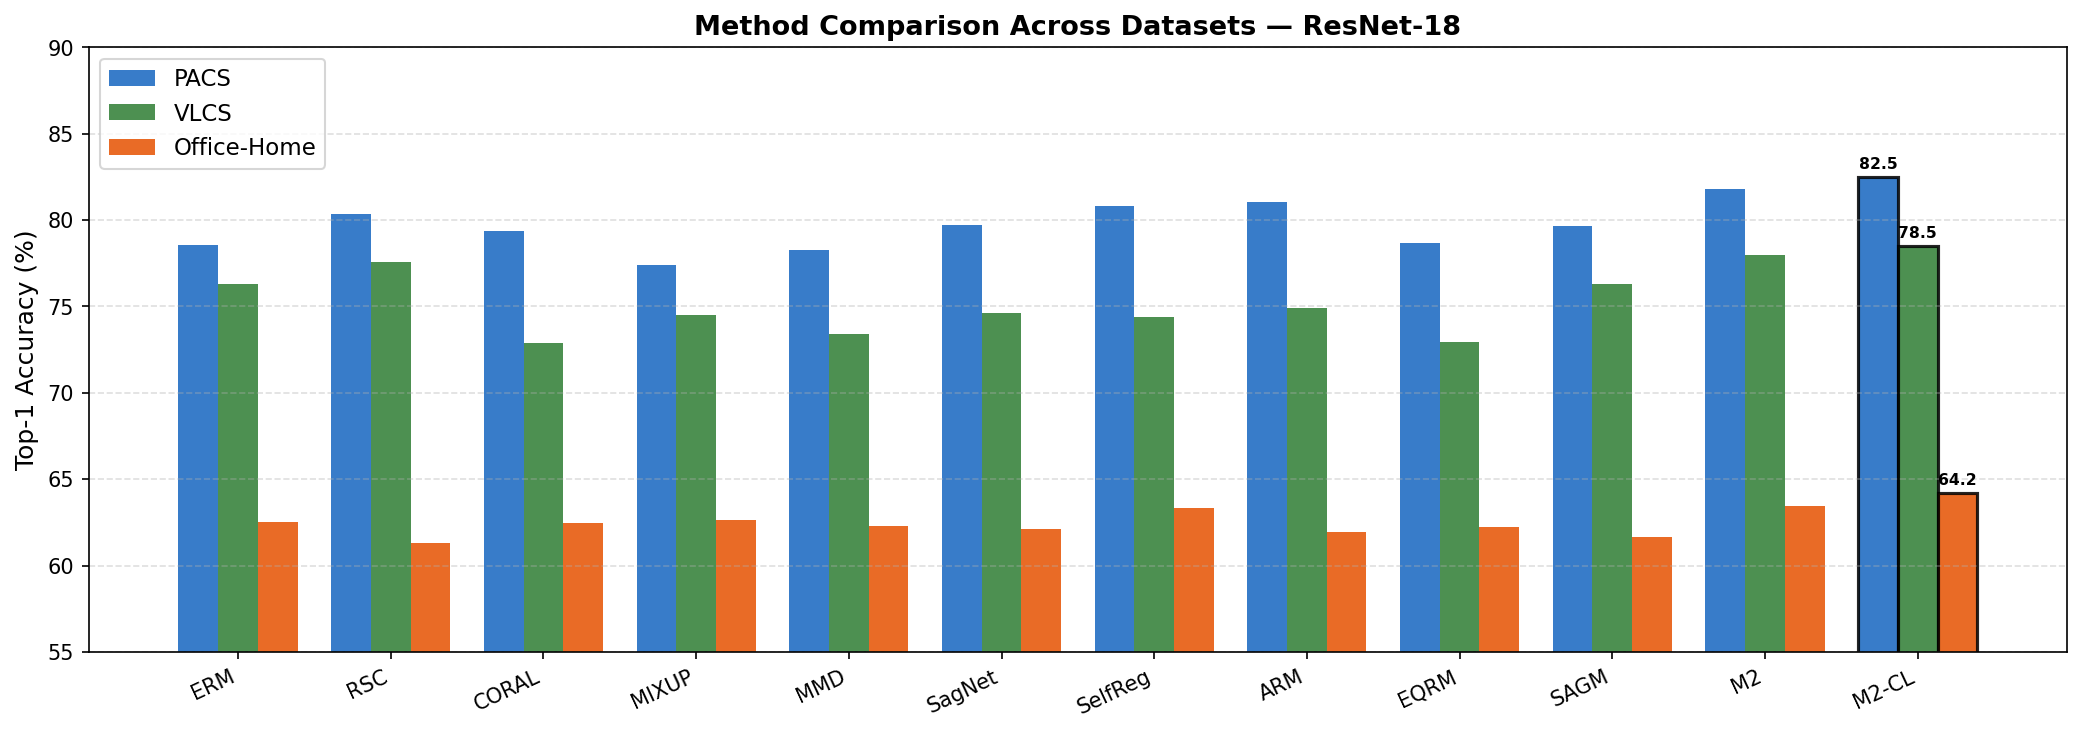
\includegraphics[width=0.95\linewidth]{photos/bar_comparison.png}
		\end{figure}
	\end{frame}

	\begin{frame}{Per-Domain Analysis on PACS (ResNet-18)}
		\begin{columns}[T]
			\begin{column}{0.5\textwidth}
				\begin{figure}
					\centering
					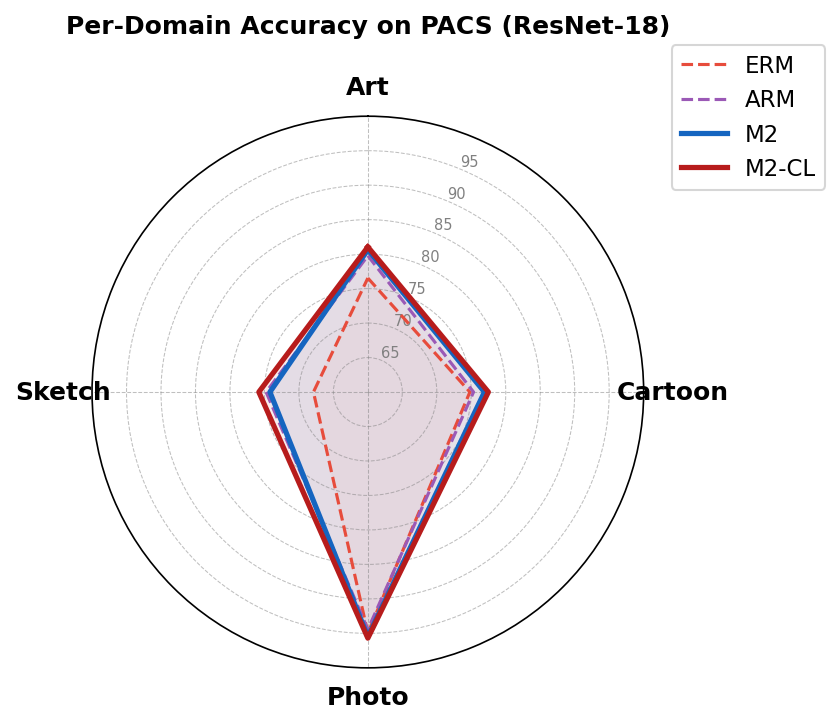
\includegraphics[width=\linewidth]{photos/radar_pacs.png}
				\end{figure}
			\end{column}
			\begin{column}{0.5\textwidth}
				\begin{block}{Key Observations}
					\begin{itemize}
						\item $M^2$-CL dominates \textbf{all four} domains simultaneously.
						\item Largest gain: \textbf{Sketch} (+7.9 pp over ERM), the hardest domain due to extreme style shift.
						\item \textbf{Art Painting} gap confirms that contrastive regularization helps most when style variance is high.
					\end{itemize}
				\end{block}
				\begin{alertblock}{Why ARM fails on Photo}
					ARM's meta-learning relies on test-time adaptation signals; \textbf{Photo} (near-real domain) provides weak adaptation gradient, reducing its advantage.
				\end{alertblock}
			\end{column}
		\end{columns}
	\end{frame}

	\begin{frame}{Quantitative Results: Main Takeaways}
		\begin{columns}[T]
			\begin{column}{0.48\textwidth}
				\begin{block}{Average Accuracy}
					\begin{itemize}
						\item \textbf{ResNet-18:} $M^2$-CL reaches \textbf{82.51} on PACS, \textbf{78.50} on VLCS, and \textbf{64.18} on Office-Home.
						\item \textbf{ResNet-50:} $M^2$-CL reaches \textbf{86.56} on PACS, \textbf{79.09} on VLCS, and \textbf{69.34} on Office-Home.
						\item The average score improves over the strongest baseline in each benchmark summary.
					\end{itemize}
				\end{block}
			\end{column}
			\begin{column}{0.48\textwidth}
				\begin{alertblock}{Interpretation}
					\begin{itemize}
						\item $M^2$ improves representation quality by reusing intermediate multi-scale features.
						\item $M^2$-CL adds class-level alignment, making same-class features closer across source domains.
						\item Per-domain scores are not uniformly best, so the ablation section checks which design choices drive the average gains.
					\end{itemize}
				\end{alertblock}
			\end{column}
		\end{columns}
	\end{frame}

	\begin{frame}{Table 5: Ablation Study on PACS and VLCS}
\begin{table}[htbp]
\centering
\caption{Ablation study on PACS and VLCS, ResNet-18.}
\tiny
\begin{adjustbox}{max width=\textwidth,max totalheight=0.72\textheight,keepaspectratio}
\begin{tabular}{llllrrrrrrrrrr}
\toprule
pipe & r & drop & loss & A & C & P & S & PACS Avg & C & L & S & V & VLCS Avg \\
\midrule
c & 2 & - & - & 72.34 & 72.29 & 94.19 & 69.51 & 78.23 & 93.87 & 60.91 & 65.89 & 61.91 & 71.22 \\
c & 4 & - & - & 74.38 & 72.74 & 90.13 & 69.71 & 77.21 & 94.14 & 59.01 & 67.82 & 65.42 & 69.62 \\
c & 6 & - & - & 75.72 & 70.12 & 94.26 & 73.33 & 77.92 & 91.93 & 56.81 & 67.28 & 64.10 & 68.95 \\
c & 2 & yes & - & 75.67 & 73.29 & 92.16 & 75.95 & 77.93 & 93.73 & 57.72 & 66.34 & 62.50 & 71.74 \\
c & 4 & yes & - & 74.36 & 74.05 & 92.57 & 76.45 & 79.37 & 96.07 & 56.28 & 67.07 & 64.30 & 65.81 \\
c & 6 & yes & - & 75.97 & 72.77 & 93.01 & 74.73 & 76.81 & 92.94 & 59.73 & 66.15 & 64.51 & 70.09 \\
p & 2 & - & - & 76.09 & 55.88 & 68.35 & 60.92 & 64.40 & 95.60 & 56.97 & 66.25 & 73.15 & 73.96 \\
p & 4 & - & - & 74.72 & 74.62 & 92.01 & 70.32 & 77.64 & 95.20 & 58.10 & 66.20 & 64.90 & 70.29 \\
p & 6 & - & - & 75.38 & 69.99 & 91.21 & 69.47 & 77.77 & 95.23 & 56.81 & 69.13 & 65.34 & 70.55 \\
p & 2 & yes & - & 74.61 & 72.39 & 87.08 & 73.95 & 78.88 & 95.73 & 58.33 & 68.44 & 63.74 & 70.49 \\
p & 6 & yes & - & 76.73 & 73.98 & 93.41 & 73.56 & 79.84 & 93.19 & 56.05 & 66.62 & 64.24 & 70.43 \\
p & 4 & yes & - & 76.39 & 75.98 & 95.58 & 74.49 & 79.15 & 94.54 & 59.77 & 67.26 & 74.55 & 73.14 \\
p & 4 & yes & yes & 80.43 & 75.43 & 96.87 & 74.42 & 80.10 & 96.09 & 61.15 & 69.05 & 75.70 & 74.15 \\
\bottomrule
\end{tabular}
\end{adjustbox}
\end{table}
	\end{frame}

	\begin{frame}{Table 6: Sensitivity to Temperature $\tau$}
\begin{table}[htbp]
\centering
\caption{Sensitivity analysis for $\tau$ in M2-CL, ResNet-18.}
\scriptsize
\begin{tabular}{lrr}
\toprule
$\tau$ & PACS & VLCS \\
\midrule
0.01 & 78.10 & 76.15 \\
0.1 & 80.03 & 77.27 \\
0.2 & 81.37 & 74.71 \\
0.4 & 82.07 & 72.03 \\
0.6 & 83.70 & 74.15 \\
0.8 & 84.67 & 75.21 \\
1.0 & 80.07 & 76.24 \\
1.2 & 81.34 & 75.11 \\
1.4 & 83.14 & 75.69 \\
1.6 & 82.17 & 76.84 \\
1.8 & 80.51 & 74.66 \\
2.0 & 78.72 & 74.99 \\
10.0 & 79.92 & 74.04 \\
100.0 & 81.84 & 73.74 \\
\bottomrule
\end{tabular}
\end{table}
	\end{frame}

	\begin{frame}{Table 7: Sensitivity to Loss Weight $\alpha$}
\begin{table}[htbp]
\centering
\caption{Sensitivity analysis for $\alpha$ in M2-CL, ResNet-18.}
\scriptsize
\begin{tabular}{lrr}
\toprule
$\alpha$ & PACS & VLCS \\
\midrule
0.00 & 82.76 & 72.36 \\
10e-5 & 80.41 & 73.56 \\
10e-4 & 81.17 & 73.71 \\
10e-3 & 82.29 & 74.38 \\
10e-2 & 79.70 & 73.39 \\
10e-1 & 64.04 & 55.96 \\
\bottomrule
\end{tabular}
\end{table}
	\end{frame}

	\begin{frame}{Core Ablation Analysis}
		\begin{block}{Table 5 Reference Insights (PACS / VLCS, ResNet-18)}
			\begin{itemize}
				\item \textbf{Best full configuration:} $p, r=4, drop=yes, loss=yes$ reaches \textbf{80.10} PACS Avg and \textbf{74.15} VLCS Avg.
				\item \textbf{Contrastive loss contribution:} adding the loss to the same $p, r=4, drop=yes$ setting improves PACS from \textbf{79.15} to \textbf{80.10} and VLCS from \textbf{73.14} to \textbf{74.15}.
				\item \textbf{Spatial dropout effect:} for $p, r=4$, dropout improves PACS from \textbf{77.64} to \textbf{79.15} and VLCS from \textbf{70.29} to \textbf{73.14}.
			\end{itemize}
		\end{block}
	\end{frame}

	\begin{frame}{Sensitivity Analysis: Loss Scaling ($\alpha$ \& $\tau$)}
		\begin{block}{Tables 6--7 Insights: Hyperparameter Tuning}
			\begin{itemize}
				\item \textbf{Temperature optimum:} PACS peaks at \textbf{84.67} with $\tau=0.8$, while VLCS peaks at \textbf{77.27} with $\tau=0.1$.
				\item \textbf{Default-scale behavior:} $\tau=1.0$ remains competitive with \textbf{80.07} PACS and \textbf{76.24} VLCS.
				\item \textbf{Loss-weight sensitivity:} $\alpha=10e^{-3}$ gives the best VLCS score, \textbf{74.38}, while $\alpha=0$ gives the highest PACS score, \textbf{82.76}.
			\end{itemize}
		\end{block}
		\begin{alertblock}{Alpha Bounds Limits }
			\[ \alpha = 10e^{-1} \implies \text{PACS } 64.04,\quad \text{VLCS } 55.96 \]
			A large contrastive weight dominates cross-entropy optimization and causes a sharp drop compared with the best scores in Table 7.
		\end{alertblock}
	\end{frame}

	% =================================================================
	% SECTION 7: QUALITATIVE VISUALIZATIONS
	% =================================================================
\section{Qualitative Visualizations}

\begin{frame}{Feature Space Visualization: ERM vs $M^2$-CL}
	\begin{figure}
		\centering
		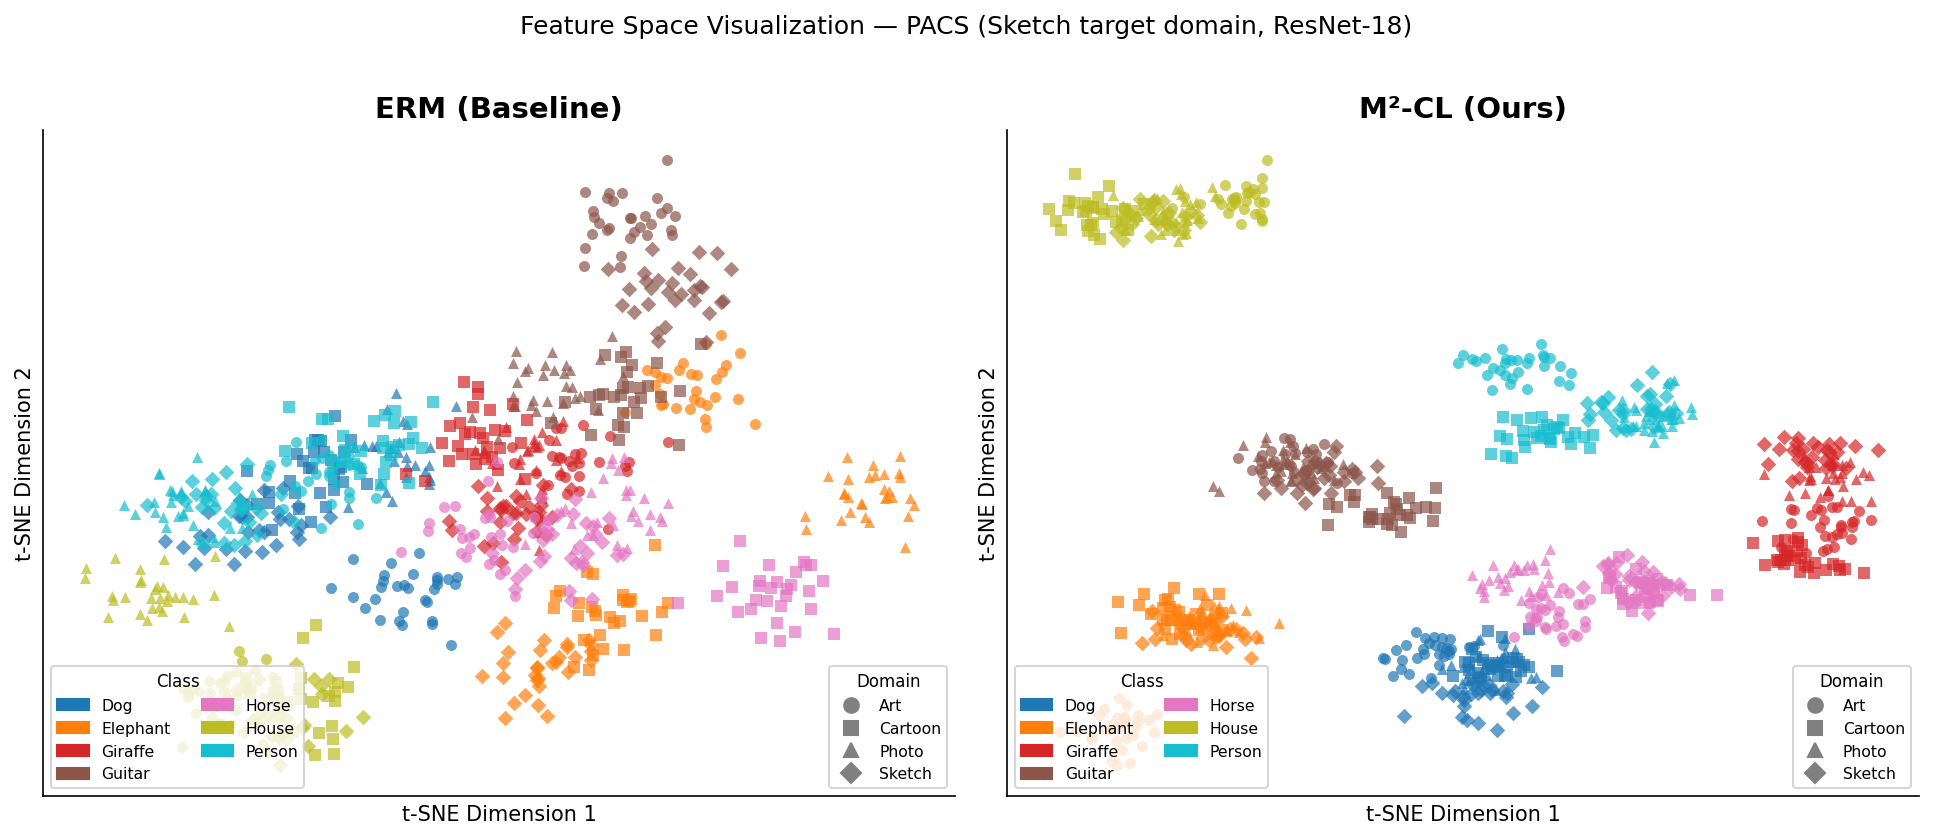
\includegraphics[width=0.95\linewidth]{photos/tsne_comparison.png}
	\end{figure}
	\vspace{-0.3cm}
	\begin{block}{}
		\small \textbf{Left (ERM):} Same-class features from different domains are dispersed — the model learns domain-specific patterns.
		\textbf{Right ($M^2$-CL):} Contrastive regularization \alert{collapses domain scatter} within each class while \alert{separating} inter-class clusters.
	\end{block}
\end{frame}

\begin{frame}{Visualizing Robustness via Saliency Maps}
	\begin{block}{Methodology}
		Visualizes the gradients of the class score function relative to input image pixels. Darker pixel weights highlight the regions that contribute most to final classification decisions.
	\end{block}

	\begin{figure}
		\centering
		
\includegraphics[width=0.78\linewidth]{photos/Pacs.png}

		\caption{Saliency maps comparison on the PACS dataset.}
	\end{figure}
\end{frame}

	\begin{frame}{Saliency Map Insights \& Interpretations}
		\begin{columns}[T]
			\begin{column}{0.5\textwidth}
				\begin{block}{Baseline ERM Traps}
					\begin{itemize}
						\item Strongly influenced by background noise and spurious environmental features (e.g., sky, roads, grass).
						\item Often focuses on non-causal elements within the scene, such as a motorcycle rider.
					\end{itemize}
				\end{block}
			\end{column}
			\begin{column}{0.5\textwidth}
				\begin{alertblock}{Proposed $M^2$-CL Solution}
					\begin{itemize}
						\item Successfully ignores irrelevant background styles and focus fields.
						\item Accurately isolates the core structural contours of objects, even in highly stylized domains like Sketch and Cartoon.
					\end{itemize}
				\end{alertblock}
			\end{column}
		\end{columns}
	\end{frame}

	% =================================================================
	% SECTION 8: CONCLUSION
	% =================================================================
	\section{Conclusion}

	\begin{frame}{Summary of Key Contributions}
		\begin{block}{Core Achievements}
			\begin{itemize}
				\item \textbf{Architecture:} Successfully combines multi-scale, multi-layer intermediate features without propagating domain-specific styles through the network.
				\item \textbf{Loss Optimization:} Introduces a layer-wise contrastive loss that enforces domain invariance across all extraction levels.
				\item \textbf{Empirical Validation:} Outperforms previous domain generalization methods and sets a new state-of-the-art across four major benchmark datasets.
			\end{itemize}
		\end{block}
	\end{frame}

	\begin{frame}{Limitations \& Future Directions}
		\begin{block}{Current Computational Drawbacks}
			\begin{itemize}
				\item \textbf{Memory Overhead:} Concatenating multiple intermediate feature maps creates dense hypercolumns before the classification head, increasing memory usage.
				\item \textbf{Batch Size Dependency:} Like most contrastive methods, $M^2$-CL requires large training batches to construct effective positive/negative pairs.
			\end{itemize}
		\end{block}
		\begin{alertblock}{Future Research Avenues}
			Explore cross-layer attention mechanics, build causal inference systems, and evaluate alternative similarity metrics like KL divergence to refine latent distribution shapes.
		\end{alertblock}
	\end{frame}

	% % =================================================================
	% % REFERENCES
	% % =================================================================
	% \useStyleLogoOnly
	% \setbeamertemplate{bibliography item}[text]

	% \begin{frame}[allowframebreaks]{References}
	% 	\begin{thebibliography}{99}
	% 		\bibitem{m2cl}
	% 		A.~Ballas and C.~Diou,
	% 		``Multiscale and Multilayer Contrastive Learning for Domain Generalization,''
	% 		\emph{IEEE Transactions on Artificial Intelligence}, March 2024[cite: 4].

	% 		\bibitem{domainbed}
	% 		I.~Gulrajani and D.~Lopez-Paz,
	% 		``In Search of Lost Domain Generalization,''
	% 		in \emph{ICLR}, 2021[cite: 688].

	% 		\bibitem{resnet}
	% 		K.~He, X.~Zhang, S.~Ren, and J.~Sun,
	% 		``Deep Residual Learning for Image Recognition,''
	% 		in \emph{CVPR}, pp.~770--778, 2016[cite: 683].

	% 		\bibitem{spatialdropout}
	% 		J.~Tompson, R.~Goroshin, A.~Jain, Y.~LeCun, and C.~Bregler,
	% 		``Efficient Object Localization Using Convolutional Networks,''
	% 		in \emph{CVPR}, pp.~648--656, 2015[cite: 590, 591].
	% 	\end{thebibliography}
	% \end{frame}

	% Closing Page
	\hustthankyou

\end{document}
